\section{回路の過渡現象・電気振動と交流の基礎}

% ===========================================================================
%  再編（2026-09-24）：第4章 電磁気学 の第31回．
%  原本の 第39回の 39.3（コイルを含む回路の過渡現象）と，第40回「振動回路・交流回路(1)」の全体
%  （40.1 電気振動／40.2 交流電圧・交流電流／40.3 抵抗／40.4 コイル／40.5 コンデンサー）を
%  合流させて1回とした（`saihen/電磁気_例題配分.md` の「第30回と第31回の境界」の通り）．
%
%  ・練習は9題．練習番号は第30回（［99］〜［110］）の続き．
%      ［111］＝㊵[78]（A問題）  ［112］＝㊴[72]（自己誘導起電力）  ［113］＝㊴[75]（RL過渡・指定）
%      ［114］＝㊵[79]（LC電気振動・指定）  ［115］＝㊵[80]（交流発電機）  ［116］＝㊵[81]（力率）
%      ［117］＝㊵[82]（素子の電圧と電流・指定）
%      C問題 ［118］＝㊵[83]（中心のずれた電気振動）  ［119］＝㊵[84]（素子にかかる電圧）
%
%  ・例題は5題．原本の 例題36・39・40・41・42．第30回が【例題30】〜【例題34】なので
%    \setcounter{nombre}{34} として【例題35】〜【例題39】と表示される．
%
%  ・【重要】原本の講義編は Google Drive の OCR テキストしか取れなかったので，例題の問題文は
%    OCR から復元し，図は circuitikz で描き起こした（`mkfig_new31ex.py`）．要照合：
%      ・例題35（原本36）：OCR では (3) の操作が「スイッチ』を閉じ，その後スイッチトを開いた」と崩れている．
%        「$\mathrm{S}_2$ を閉じ，その後 $\mathrm{S}_1$ を開いた」と判断し，$\mathrm{S}_2$ は抵抗とコイルを電池から切り離して
%        閉じたループをつくる位置に描いた．
%      ・例題36（原本39）：OCR の通り (1)〜(8)．電流の正の向きは OCR「反時計まわり」→ 図に合わせて
%        「コンデンサーの上側極板から流れ出てコイルへ向かう向き」とした．
%      ・例題38・39（原本41・42）：電源電圧は OCR の通り $V_0\cos\omega t$．
%    原本には例題の解答が無いので，指針・解答はすべて書き起こした．
%
%  ・原本の本文に無く，練習・例題が前提にしていたものを加筆した：
%      ・31.1 に{RC 回路との比較}（コイルは電流を，コンデンサーは電荷を急に変えない）と時定数 $\frac{L}{R}$．
%      ・31.2 に{電気振動のエネルギー保存}と{単振動との対応}（練習［114］［118］の注・参考）．
%      ・31.7 を新設：{一般の素子の平均電力と力率} $\overline{P}=V_{\mathrm{e}}I_{\mathrm{e}}\cos\varphi$
%        （練習［116］．再編案「電圧と電流の瞬時値から平均電力・力率を求める説明を置く」）．
%      ・旧 `physics_ch40.tex` の誤植 $V(t)=V_0\sin(\omega T+\varphi)$（大文字 $T$）と
%        「コイルの両端にかかる交流電流$V(t)$」（電圧）を直した．
%
%  ・原本（問題編の解答）の誤りを直した（いずれもコメントで明記）：
%      (a) 練習［111］(4) の解答の式「$2\cdot 3.14\cdot 100\cdot(100\times 10^{-6})$」→ $10\times 10^{-6}$
%          （問題文は $10\U{\mu F}$．答の $1.59\times 10^2$ は $10\U{\mu F}$ の値で正しい）．
%      (b) 練習［111］の解答で誘導・容量リアクタンスを $Z_{\mathrm{L}}$，$Z_{\mathrm{C}}$ と書いていた → $X_L$，$X_C$．
%      (c) 旧回の番号による参照（「B問題［40］」「B問題［41］の注意」「B問題［31］」「→［30］」）を付け替えた．
%
%  ・図：講義の図は講義編から切り出し済みのもの（img/text/text2_p80〜p87）．
%    練習・解答の図は `mkfig_new31.py`＋`jobs_new31.py`，例題の図は `mkfig_new31ex.py`．
% ===========================================================================

% 例題番号：第30回が【例題30】〜【例題34】
\setcounter{nombre}{34}

\subsection{コイルを含む回路の過渡現象}

第30回で見たように，コイルは{\gtfamily 自分に流れる電流の変化を妨げる}素子である．
そのため，直流回路にコイルが含まれていると，スイッチを入れても電流はすぐには変化せず，しだいに変化して定常状態に近づく．
この様子は，キルヒホッフの第二法則にコイルの自己誘導起電力$-L\dfrac{dI}{dt}$を入れた式から定性的に説明できる（例題35）．

% 加筆：RC との比較（第27回 27.3）と時定数．
第27回で学んだコンデンサーの過渡現象と比べると，次のように対になっている．
\begin{description}
\item[\MARU{1}] スイッチ操作の直前・直後で，{\gtfamily コンデンサーの電荷}は変わらない ／ {\gtfamily コイルを流れる電流}は変わらない．
\item[\MARU{2}] 十分時間が経つと，コンデンサーには電流が流れない（切れた導線と同じ） ／ コイルには電圧がかからない（ただの導線と同じ）．
\end{description}
したがって，電流$0$のコイルはスイッチを入れた直後は「切れた導線」のようにふるまい，十分時間が経つと「抵抗$0$の導線」になる．
$R$と$L$の直列回路では電流は$I=\dfrac{V}{R}\bigl(1-e^{-\frac{R}{L}t}\bigr)$のように変化し，$\dfrac{L}{R}$（単位は$\U{s}$）が{\gtfamily 時定数}である（RC 回路の$RC$に対応する）．

\bsNeed{30mm}
\begin{matome}{コイルを含む直流回路}
 \hspace{3mm} スイッチ操作の直前直後：\AnaB{コイルを流れる電流は変わらない}\\
 \hspace{3mm} 十分時間が経過した後：\AnaB{コイルの両端の電圧は$0$}（電流が一定なので自己誘導起電力が生じない）
\end{matome}

%%%%%%%%%%  例題35（原本の【例題36】）  %%%%%%%%%%%%%%%%%%%%
\bsNeed{60mm}
\begin{reidaiunit}
\begin{reidai}{コイルを含む直流回路}
\begin{zuright}{62mm}
\hspace{1zw}内部抵抗の無視できる起電力$V\U{V}$の電池，抵抗値$R\U{\Omega}$の電気抵抗，自己インダクタンス$L\U{H}$のコイル，スイッチ$\mathrm{S}_1$，$\mathrm{S}_2$を組み合わせて図のような回路を作る．図の矢印の向きにコイルを流れる電流を$I\U{A}$とし，スイッチははじめすべて開いているものとする．以下の問いに答えよ．
\zusep
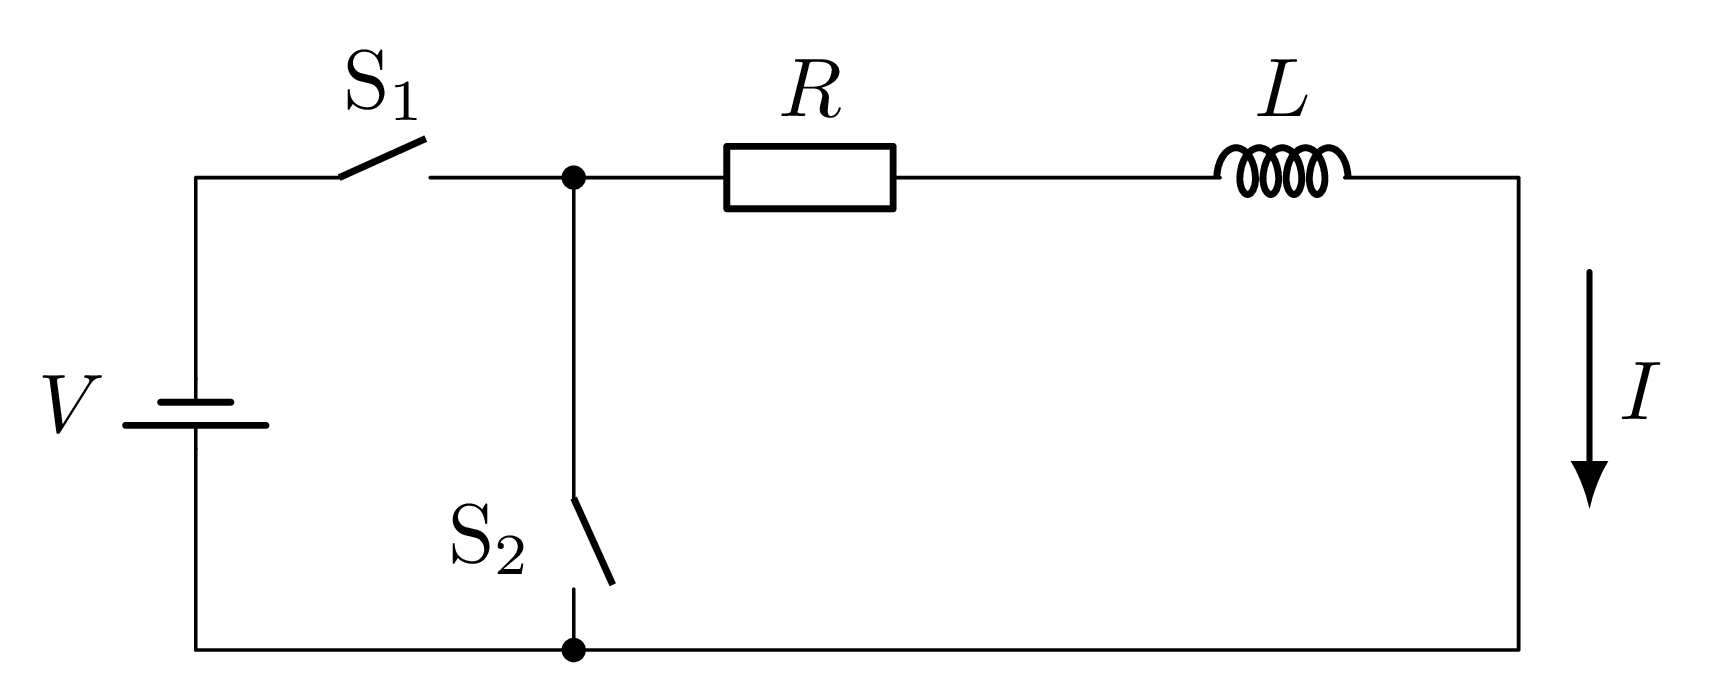
\includegraphics[keepaspectratio,width=62mm]{fig/n31_ex35_zu.png}
\end{zuright}
\begin{komon}
\ko{1} まず，スイッチ$\mathrm{S}_1$を閉じる．このとき，キルヒホッフの法則を用いて回路に成り立つ関係式を立てよ．
\ko{2} (1)を元に，電流がこの後どのように時間変化するかを述べ，式から定常状態において流れる電流$I_1\U{A}$を求めよ．
\ko{3} (2)の定常状態に至ったのち，スイッチ$\mathrm{S}_2$を閉じ，その後スイッチ$\mathrm{S}_1$を開いた．このとき，キルヒホッフの法則を用いて回路に成り立つ関係式を立てよ．
\ko{4} (3)の式を元に，電流がこの後どのように時間変化するかを述べ，式から定常状態において流れる電流$I_2\U{A}$を求めよ．
\end{komon}
\end{reidai}

\begin{sisinE}
コイルは電流の向きを正として$-L\dfrac{dI}{dt}$の起電力をもつ電池とみなす．
第二法則の式を$\dfrac{dI}{dt}=\cdots$の形に直すと，$I$が増えるか減るか，いつ止まるかが読み取れる．
定常状態では$\dfrac{dI}{dt}=0$である．
\end{sisinE}

\Key{自己誘導起電力$-L\dfrac{dI}{dt}$\quad コイルの電流は急には変わらない\quad 定常状態では$\dfrac{dI}{dt}=0$}

\begin{kaitou}
\begin{komon}
\ko{1} 電池・抵抗・コイルのループについて
       \Ana{V-L\frac{dI}{dt}=RI\Ans}
\ko{2} (1)より$\dfrac{dI}{dt}=\dfrac{V-RI}{L}$．はじめ$I=0$なので$\dfrac{dI}{dt}=\dfrac{V}{L}>0$で電流は増えはじめるが，$I$が増えるほど増加率は小さくなり，$\dfrac{dI}{dt}=0$となる値に近づく．よって定常状態の電流は
       \[I_1=\frac{V}{R}\U{A}\Ans\]
\ko{3} $\mathrm{S}_2$を閉じて$\mathrm{S}_1$を開くと，電池が切り離され，抵抗・コイル・$\mathrm{S}_2$のループだけが残る．コイルの電流は急には変わらないので，直後もこのループに$I_1$が流れている．第二法則より
       \Ana{-L\frac{dI}{dt}=RI\Ans}
\ko{4} $\dfrac{dI}{dt}=-\dfrac{R}{L}I<0$なので電流は減少していき，減少率もしだいに小さくなって$0$に近づく．定常状態では
       \[I_2=0\U{A}\Ans\]
       \begin{chuu}
       (3)の間に抵抗で発生するジュール熱の合計は，はじめにコイルに蓄えられていたエネルギー$\dfrac{1}{2}LI_1^2=\dfrac{LV^2}{2R^2}$に等しい．
       \end{chuu}
\end{komon}
\end{kaitou}
\end{reidaiunit}

\subsection{電気振動}

コンデンサーとコイルをループ状につないだ回路（{\gtfamily LC回路}）では，コンデンサーの電荷と回路を流れる電流が周期的に変化する．これを{\gtfamily 電気振動}という．
下図のように，(a)充電されたコンデンサーから電荷が流れ出して電流となり，(b)(c)コイルがその電流を流し続けようとするので，極板の電荷が逆向きに充電され，(d)(e)同じことが逆向きに繰り返される．

\begin{center}

\includegraphics[keepaspectratio,width=118mm]{text2_p80_fig1.png}
\end{center}

コンデンサーの電荷を$Q$，回路の電流を$I=-\dfrac{dQ}{dt}$とすると，第二法則$-L\dfrac{dI}{dt}=-\dfrac{Q}{C}$より
\[\frac{d^2Q}{dt^2}=-\frac{1}{LC}Q\]
となる．これは単振動の運動方程式$\dfrac{d^2x}{dt^2}=-\omega^2x$と同じ形なので，$Q$は角周波数$\omega=\dfrac{1}{\sqrt{LC}}$で振動する．周波数は
\AnaBD{f=\frac{1}{2\pi\sqrt{LC}}\U{Hz}}
であり，これを回路の{\gtfamily 固有周波数}という．

% 加筆：エネルギー保存と単振動との対応（練習［114］［118］）．
抵抗がなければエネルギーは失われず，コンデンサーの静電エネルギーとコイルの磁場のエネルギーの和が一定に保たれる：
\[\frac{Q^2}{2C}+\frac{1}{2}LI^2=\text{一定}\]
電荷が最大のとき電流は$0$，電流が最大のとき電荷は$0$である．
単振動との対応は，$Q\leftrightarrow x$，$I\leftrightarrow v$，$L\leftrightarrow m$，$\dfrac{1}{C}\leftrightarrow k$である（$\omega=\sqrt{\dfrac{k}{m}}\leftrightarrow\dfrac{1}{\sqrt{LC}}$）．
単振動で振動の中心がずれることがあったように，電気振動でも$\dfrac{d^2Q}{dt^2}=-\omega^2(Q-Q_{\mathrm{c}})$の形になれば$Q_{\mathrm{c}}$を中心に振動する（練習［118］）．

\bsNeed{30mm}
\begin{matome}{電気振動}
 \hspace{3mm} $\dfrac{d^2Q}{dt^2}=-\dfrac{1}{LC}Q$\quad 角周波数$\omega=\dfrac{1}{\sqrt{LC}}$，周期$T=2\pi\sqrt{LC}$\\
 \hspace{3mm} エネルギー保存\quad $\dfrac{Q^2}{2C}+\dfrac{1}{2}LI^2=$一定
\end{matome}

%%%%%%%%%%  例題36（原本の【例題39】）  %%%%%%%%%%%%%%%%%%%%
\bsNeed{90mm}
\begin{reidaiunit}
\begin{reidai}{電気振動}
\begin{zuright}{46mm}
\hspace{1zw}内部抵抗の無視できる起電力$V\U{V}$の電池，電気容量$C\U{F}$のコンデンサー，自己インダクタンス$L\U{H}$のコイルを図のように接続した．初め，コンデンサーには電荷が蓄えられていないものとして以下の設問に答えよ．
\zusep
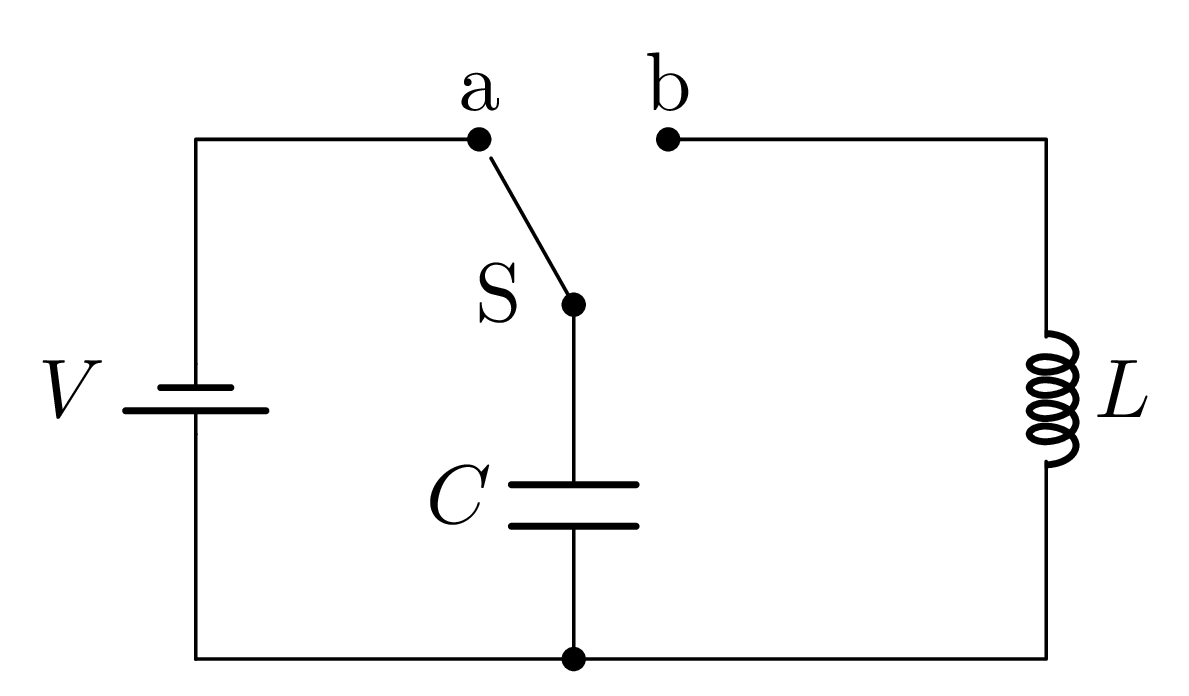
\includegraphics[keepaspectratio,width=44mm]{fig/n31_ex36_zu.png}
\end{zuright}
\begin{komon}
\ko{1} まず，スイッチ$\mathrm{S}$を$\mathrm{a}$側に接続して十分時間を経過させた．このとき，コンデンサーの上側極板に蓄えられる電荷$Q_0\U{C}$を求めよ．
\ko{2} 続いて時刻$t=0$にスイッチ$\mathrm{S}$を$\mathrm{b}$に接続すると，電気振動が生じた．時刻$t$においてコンデンサーの上側極板に蓄えられている電荷を$Q\U{C}$，LC回路部分に流れている電流を$I\U{A}$（ただしコンデンサーの上側極板から流れ出てコイルへ向かう向きを正とする）とおく．このとき，キルヒホッフの第二法則を用いて$Q$，$I$，$C$，$L$の間に成り立つ関係を表せ．
\ko{3} $Q$と$I$との間に成立する関係式を，微分を用いて表せ．
\ko{4} (2)(3)より，$I$を含まない$Q$に関する微分方程式を立てよ．
\ko{5} (4)の微分方程式を元に，この電気振動の角周波数$\omega\U{rad/s}$，周波数$f\U{Hz}$，周期$T\U{s}$を求めよ．
\ko{6} $t=0$で$Q=Q_0$，$I=0$であることから，時刻$t$における$Q$の値を求めよ．
\ko{7} (3)(6)を用いて，時刻$t$における$I$の値を求めよ．
\ko{8} コンデンサーに蓄えられるエネルギー$\dfrac{Q^2}{2C}$とコイルに蓄えられるエネルギー$\dfrac{1}{2}LI^2$の和が時刻によらず一定となっていることを示せ．
\end{komon}
\end{reidai}

\begin{sisinE}
(3) 正の向きの電流$I$が流れると上側極板の電荷$Q$は減る．
(4)(5) 単振動の運動方程式$\dfrac{d^2x}{dt^2}=-\omega^2x$と比べる．
(6) $t=0$で最大値$Q_0$から始まる単振動なので$\cos$で書ける．
\end{sisinE}

\Key{微分方程式$\dfrac{d^2Q}{dt^2}=-\omega^2Q$ → $Q$は角周波数$\omega$の単振動\quad コイルに蓄えられるエネルギー$\dfrac{1}{2}LI^2$}

\begin{kaitou}
\begin{komon}
\ko{1} 十分時間が経つとコンデンサーの電圧は$V$になるので
       \[Q_0=CV\U{C}\Ans\]
\ko{2} コンデンサーを起電力$\dfrac{Q}{C}$の電池とみなすと，LCのループについて
       \Ana{\frac{Q}{C}-L\frac{dI}{dt}=0\Ans}
\ko{3} \[I=-\frac{dQ}{dt}\Ans\]
\ko{4} (3)を微分して(2)に代入すると
       \[\frac{d^2Q}{dt^2}=-\frac{1}{LC}Q\Ans\]
\ko{5} 単振動の式と比べて
       \Ana{\omega=\frac{1}{\sqrt{LC}},\quad f=\frac{1}{2\pi\sqrt{LC}},\quad T=2\pi\sqrt{LC}\Ans}
\ko{6} $t=0$で最大値$CV$から始まるので
       \[Q=CV\cos\frac{t}{\sqrt{LC}}\U{C}\Ans\]
\ko{7} \[I=-\frac{dQ}{dt}=V\sqrt{\frac{C}{L}}\sin\frac{t}{\sqrt{LC}}\U{A}\Ans\]
       \begin{center}\AnaFig{50mm}{fig/n31_ex36_ans.png}{fig/n31_ex36_ans_blank.png}\end{center}
\ko{8} \[\frac{Q^2}{2C}+\frac{1}{2}LI^2=\frac{CV^2}{2}\cos^2\frac{t}{\sqrt{LC}}+\frac{CV^2}{2}\sin^2\frac{t}{\sqrt{LC}}=\frac{1}{2}CV^2\]
       となり，時刻によらず一定である．\Ans
\end{komon}
\end{kaitou}
\end{reidaiunit}

\subsection{交流電圧・交流電流}

家庭用電源として送られているのは，電池のような直流電圧ではなく{\gtfamily 交流電圧}である．
交流電圧は端子間の電圧が一定ではなく，時間に対して三角関数的に変化する電圧であり，時刻$t$の電圧が
\[V(t)=V_0\sin(\omega t+\varphi)\U{V}\]
のように表される．
$V_0\ (>0)$を{\gtfamily 最大値}，$\omega$を{\gtfamily 角周波数}，$\varphi$を{\gtfamily 初期位相}，$V(t)$を{\gtfamily 瞬時値}という．周波数は$f=\dfrac{\omega}{2\pi}$，周期は$T=\dfrac{2\pi}{\omega}$である．

\begin{zuright}{50mm}
\hspace{1zw}交流電圧は，図のように磁場中でコイルを一定の角速度で回転させることにより発生させることができる．
磁束密度$B$の一様な磁場中で，面積$S$のコイルが角速度$\omega$で回転し，時刻$0$で磁場に垂直であったとすると，時刻$t$でコイルを貫く磁束は
\[\varPhi=BS\cos\omega t\]
であり，コイルに生じる誘導起電力は
\[V=-\frac{d\varPhi}{dt}=\omega BS\sin\omega t\]
となって，三角関数的に変化する電圧が得られる（練習［115］）．
\zusep

\includegraphics[keepaspectratio,width=48mm]{text2_p82_fig1.png}\\[2mm]

\includegraphics[keepaspectratio,width=48mm]{text2_p82_fig2.png}
\end{zuright}

このような交流電圧を抵抗・コイル・コンデンサーに接続すると，素子には同じ角周波数で三角関数的に変化する{\gtfamily 交流電流}$I(t)=I_0\sin(\omega t+\varphi^\prime)$が流れる．
以下では，素子ごとに{\gtfamily 最大値の関係}と{\gtfamily 位相の関係}を調べる．

\subsection{抵抗にかかる交流電圧と交流電流}

\begin{zuright}{40mm}
\hspace{1zw}抵抗の両端に交流電圧$V(t)=V_0\sin(\omega t+\varphi)$がかかると，オームの法則$V(t)=RI(t)$より
\[I(t)=\frac{V_0}{R}\sin(\omega t+\varphi)\]
の電流が流れる．最大値の間には
\AnaBD{V_0=RI_0}
が成り立ち，位相は同じ（電圧と電流が同時に最大になる）．これを{\gtfamily 電圧と電流に位相差がない}という．

\hspace{1zw}時刻$t$の消費電力は
\[P(t)=V(t)I(t)=\frac{V_0I_0}{2}\{1-\cos 2(\omega t+\varphi)\}\]
で，図のように時間変動するが，平均すると$\overline{P}=\dfrac{V_0I_0}{2}$である．交流で単に「電力」と呼ぶときはこの平均値をさす．
\zusep

\includegraphics[keepaspectratio,width=34mm]{text2_p83_fig1.png}
\end{zuright}

ここで，最大値の$\dfrac{1}{\sqrt{2}}$倍を{\gtfamily 実効値}と定義する：
\AnaBD{V_{\mathrm{e}}=\frac{V_0}{\sqrt{2}},\qquad I_{\mathrm{e}}=\frac{I_0}{\sqrt{2}}}
すると$\overline{P}=V_{\mathrm{e}}I_{\mathrm{e}}=RI_{\mathrm{e}}^2=\dfrac{V_{\mathrm{e}}^2}{R}$と，直流と同じ形の式で書けるので便利である．
交流で単に「電圧」「電流」という場合は実効値をさす．家庭の交流電圧$100\U{V}$も実効値である．

\bsNeed{36mm}
\begin{matome}{実効値・抵抗の交流}
 \hspace{3mm} 実効値：最大値の$\dfrac{1}{\sqrt{2}}$倍\quad $V_{\mathrm{e}}=\dfrac{V_0}{\sqrt{2}}$，$I_{\mathrm{e}}=\dfrac{I_0}{\sqrt{2}}$\qquad 消費電力（時間平均）$\overline{P}=\dfrac{V_0I_0}{2}=V_{\mathrm{e}}I_{\mathrm{e}}$\\
 \hspace{3mm} 抵抗：$V_0=RI_0$（実効値でも$V_{\mathrm{e}}=RI_{\mathrm{e}}$）．電圧と電流の位相は\AnaB{一致する}
\end{matome}

%%%%%%%%%%  例題37（原本の【例題40】）  %%%%%%%%%%%%%%%%%%%%
\bsNeed{56mm}
\begin{reidaiunit}
\begin{reidai}{抵抗にかかる交流電圧と交流電流}
\hspace{1zw}関東地区で家庭に供給されている電気は，周波数$50\U{Hz}$，電圧$100\U{V}$の交流電圧である．
\begin{komon}
\ko{1} この交流電圧の最大値を求めよ．
\ko{2} 時刻$t=0$に交流電圧が最大値をとった．このとき，この交流電圧の時間変化を表す式を書け．
\ko{3} この交流電圧に$50\U{\Omega}$の抵抗を接続した．このとき，この抵抗に流れる電流の実効値，および時刻$t$における瞬時値を求めよ．
\end{komon}
\end{reidai}

\begin{sisinE}
「交流電源の$100\U{V}$」とは電圧の実効値である．交流において電圧・電流という場合は実効値を意味する．
抵抗では電圧と電流の位相が一致する．
\end{sisinE}

\Key{実効値$V_{\mathrm{e}}=\dfrac{V_0}{\sqrt{2}}$\quad 抵抗では$V_0=RI_0$，位相は一致}

\begin{kaitou}
\begin{komon}
\ko{1} \[V_0=\sqrt{2}\times 100\fallingdotseq 141\U{V}\Ans\]
\ko{2} $\omega=2\pi f=100\pi\U{rad/s}$で，$t=0$で最大なので
       \[V(t)=100\sqrt{2}\cos 100\pi t\U{V}\Ans\]
\ko{3} 実効値は
       \[I_{\mathrm{e}}=\frac{100}{50}=2.0\U{A}\Ans\]
       瞬時値は位相が電圧と同じで最大値$2\sqrt{2}\U{A}$なので
       \Ana{I(t)=2\sqrt{2}\cos 100\pi t\U{A}\Ans}
\end{komon}
\end{kaitou}
\end{reidaiunit}

\subsection{コイルにかかる交流電圧と交流電流}

\begin{zuright}{38mm}
\hspace{1zw}コイルの両端に交流電圧$V(t)=V_0\sin(\omega t+\varphi)$をかけると，第二法則$V(t)-L\dfrac{dI}{dt}=0$より$\dfrac{dI}{dt}=\dfrac{V_0}{L}\sin(\omega t+\varphi)$．
積分して，時間変化しない定数部分を$0$とすると
\[I(t)=\frac{V_0}{\omega L}\sin\Bigl(\omega t+\varphi-\frac{\pi}{2}\Bigr)\]
が流れる．最大値の間には
\AnaBD{V_0=\omega LI_0}
が成り立つ．
\hspace{1zw}グラフの凹凸に着目すると，電流の変化は電圧の変化より$\dfrac{T}{4}$だけ遅れて現れる．位相では$\dfrac{\pi}{2}$の遅れなので，{\gtfamily コイルを流れる電流の位相は，電圧の位相より$\dfrac{\pi}{2}$遅れる}．
コイルは電流の変化を嫌うので，電圧を変えても電流が遅れて変化する，と解釈できる．
\zusep

\includegraphics[keepaspectratio,width=36mm]{text2_p84_fig1.png}
\end{zuright}

$V_0=\omega LI_0$はオームの法則と同じ形なので，比例定数$X_L=\omega L\U{\Omega}$をコイルの{\gtfamily 誘導リアクタンス}という．
周波数が高いほど電流は流れにくい．
ただし，この関係は{\gtfamily 最大値（実効値）の間の関係}であり，各瞬間に$V(t)=\omega LI(t)$が成り立つのではない．
また，電圧と電流の位相が$\dfrac{\pi}{2}$ずれているので，{\gtfamily コイルの消費電力の時間平均は$0$}である（31.7）．

\bsNeed{28mm}
\begin{matome}{コイルの交流}
 \hspace{3mm} $V_0=\omega LI_0$（誘導リアクタンス$X_L=\omega L$）\qquad 電流の位相は電圧より\AnaB{$\dfrac{\pi}{2}$遅れる}\qquad 平均電力$0$
\end{matome}

%%%%%%%%%%  例題38（原本の【例題41】）  %%%%%%%%%%%%%%%%%%%%
\bsNeed{56mm}
\begin{reidaiunit}
\begin{reidai}{コイルにかかる交流電圧と交流電流}
\begin{zuright}{40mm}
\hspace{1zw}自己インダクタンスが$L\U{H}$のコイルに，図の$-$に対する$+$の電圧の瞬時値が$V(t)=V_0\cos\omega t\U{V}$で表される交流電源を接続した．このとき，以下の設問に答えよ．
\begin{komon}
\ko{1} 図の向きに流れる交流電流$I(t)$の最大値および実効値を求めよ．
\ko{2} 交流電流$I(t)$の瞬時値を求めよ．
\ko{3} コイルでの消費電力の時間平均を求めよ．
\end{komon}
\zusep
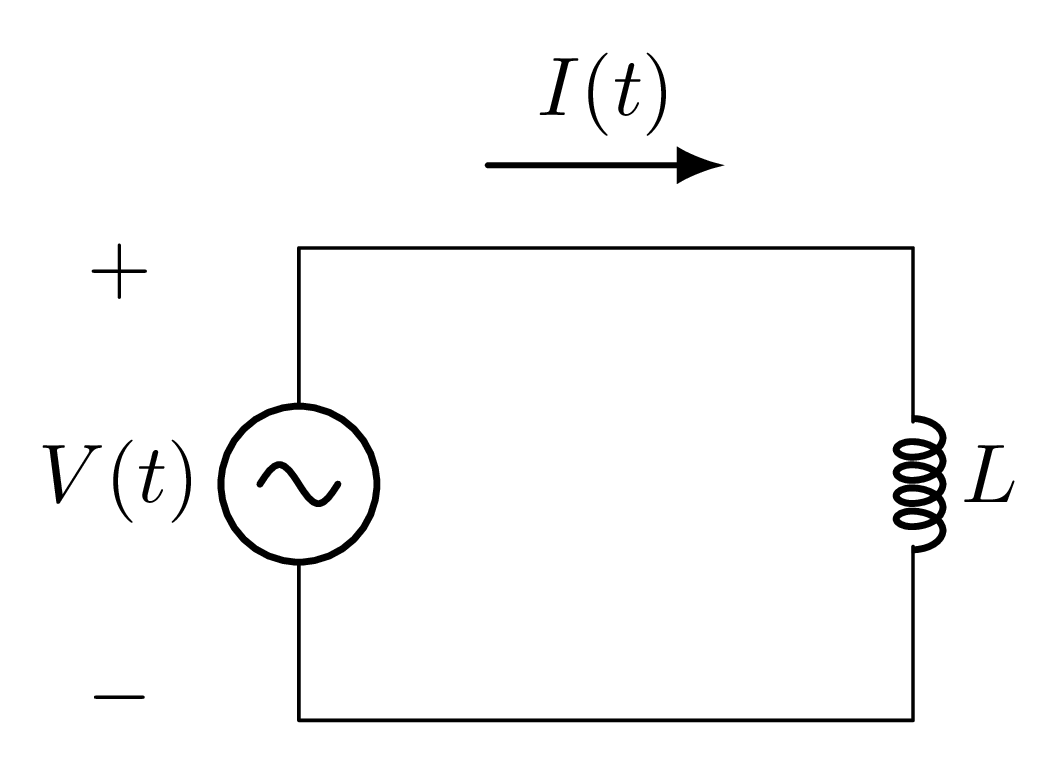
\includegraphics[keepaspectratio,width=36mm]{fig/n31_ex38_zu.png}
\end{zuright}
\end{reidai}

\begin{sisinE}
(2) コイルに流れる電流の瞬時値を求めるには，まず最大値を求め，次に位相のずれ（$\dfrac{\pi}{2}$の遅れ）を考える．
\end{sisinE}

\Key{最大値の間には$V_0=\omega LI_0$\quad 交流電流の位相は交流電圧より$\dfrac{\pi}{2}$遅れる}

\begin{kaitou}
\begin{komon}
\ko{1} \[I_0=\frac{V_0}{\omega L}\U{A},\qquad I_{\mathrm{e}}=\frac{V_0}{\sqrt{2}\,\omega L}\U{A}\Ans\]
\ko{2} 電圧の位相$\omega t$より$\dfrac{\pi}{2}$遅れるので
       \Ana{I(t)=\frac{V_0}{\omega L}\cos\Bigl(\omega t-\frac{\pi}{2}\Bigr)=\frac{V_0}{\omega L}\sin\omega t\U{A}\Ans}
\ko{3} $P(t)=V(t)I(t)=\dfrac{V_0^2}{\omega L}\sin\omega t\cos\omega t=\dfrac{V_0^2}{2\omega L}\sin 2\omega t$の時間平均は
       \[\overline{P}=0\U{W}\Ans\]
\end{komon}
\end{kaitou}
\end{reidaiunit}

\subsection{コンデンサーにかかる交流電圧と交流電流}

\begin{zuright}{38mm}
\hspace{1zw}コンデンサーの両端の電圧が$V(t)=V_0\sin(\omega t+\varphi)$のとき，電流の流れ込む極板の電荷は$Q(t)=CV(t)$である．$I(t)=\dfrac{dQ}{dt}$より
\[I(t)=C\frac{dV}{dt}=\omega CV_0\sin\Bigl(\omega t+\varphi+\frac{\pi}{2}\Bigr)\]
となる．最大値の間には
\AnaBD{V_0=\frac{1}{\omega C}I_0}
が成り立つ．
\hspace{1zw}電流の変化は電圧の変化より$\dfrac{T}{4}$早く現れる．すなわち{\gtfamily コンデンサーを流れる電流の位相は，電圧の位相より$\dfrac{\pi}{2}$進む}．
電流が流れ込んで極板に電荷がたまってから電圧が変化するので，電流の変化に遅れて電圧が変化する，と解釈できる．
\zusep

\includegraphics[keepaspectratio,width=36mm]{text2_p86_fig1.png}
\end{zuright}

比例定数$X_C=\dfrac{1}{\omega C}\U{\Omega}$をコンデンサーの{\gtfamily 容量リアクタンス}という．周波数が高いほど電流は流れやすい．
この関係も最大値（実効値）の間の関係であり，コンデンサーの消費電力の時間平均も$0$である．

\begin{zuright}{36mm}
\hspace{1zw}なお，コンデンサーの左右の極板には正負逆で大きさの等しい電荷がたまるので，左の極板に電流$I(t)$が流れ込むと，右の極板からも同じ$I(t)$が流れ出す．そのため，交流の取り扱いでは{\gtfamily 電流$I(t)$がコンデンサーを通り抜けている}と考えてよい（実際に電荷が極板の間を飛び越えているわけではない）．
\zusep

\includegraphics[keepaspectratio,width=34mm]{text2_p87_fig1.png}
\end{zuright}

\bsNeed{28mm}
\begin{matome}{コンデンサーの交流}
 \hspace{3mm} $V_0=\dfrac{1}{\omega C}I_0$（容量リアクタンス$X_C=\dfrac{1}{\omega C}$）\qquad 電流の位相は電圧より\AnaB{$\dfrac{\pi}{2}$進む}\qquad 平均電力$0$
\end{matome}

%%%%%%%%%%  例題39（原本の【例題42】）  %%%%%%%%%%%%%%%%%%%%
\bsNeed{56mm}
\begin{reidaiunit}
\begin{reidai}{コンデンサーにかかる交流電圧と交流電流}
\begin{zuright}{40mm}
\hspace{1zw}電気容量が$C\U{F}$のコンデンサーに，図の$-$に対する$+$の電圧の瞬時値が$V(t)=V_0\cos\omega t\U{V}$で表される交流電源を接続した．このとき，以下の設問に答えよ．
\begin{komon}
\ko{1} 図の向きに流れる交流電流$I(t)$の最大値および実効値を求めよ．
\ko{2} 交流電流$I(t)$の瞬時値を求めよ．
\ko{3} コンデンサーでの消費電力の時間平均を求めよ．
\end{komon}
\zusep
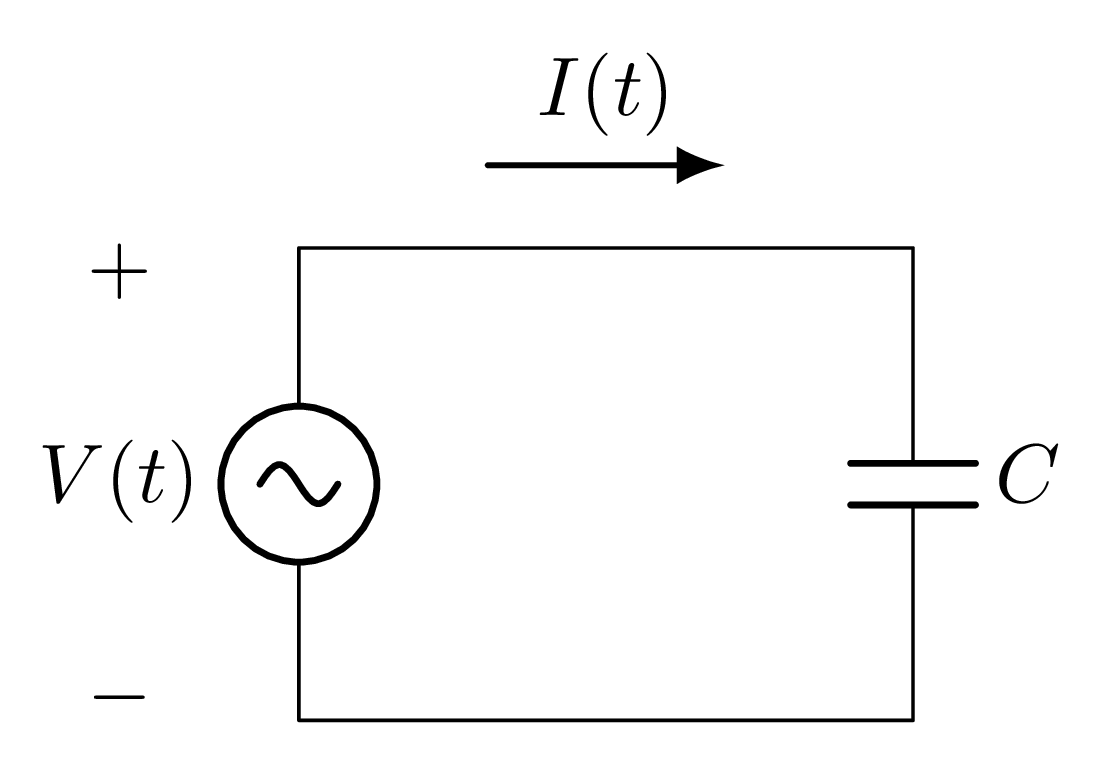
\includegraphics[keepaspectratio,width=36mm]{fig/n31_ex39_zu.png}
\end{zuright}
\end{reidai}

\begin{sisinE}
例題38と同様に，最大値 → 位相のずれ（$\dfrac{\pi}{2}$の進み）の順に考える．$I=\dfrac{dQ}{dt}=C\dfrac{dV}{dt}$を直接微分して確かめてもよい．
\end{sisinE}

\Key{最大値の間には$V_0=\dfrac{1}{\omega C}I_0$\quad 交流電流の位相は交流電圧より$\dfrac{\pi}{2}$進む}

\begin{kaitou}
\begin{komon}
\ko{1} \[I_0=\omega CV_0\U{A},\qquad I_{\mathrm{e}}=\frac{\omega CV_0}{\sqrt{2}}\U{A}\Ans\]
\ko{2} 電圧の位相より$\dfrac{\pi}{2}$進むので
       \Ana{I(t)=\omega CV_0\cos\Bigl(\omega t+\frac{\pi}{2}\Bigr)=-\omega CV_0\sin\omega t\U{A}\Ans}
       （$I=C\dfrac{dV}{dt}=-\omega CV_0\sin\omega t$と一致する．）
\ko{3} $P(t)=-\dfrac{\omega CV_0^2}{2}\sin 2\omega t$の時間平均は
       \[\overline{P}=0\U{W}\Ans\]
\end{komon}
\end{kaitou}
\end{reidaiunit}

% 加筆：一般の素子の平均電力と力率（練習［116］．再編案の指示）．
\subsection{交流の平均電力と力率}

ある素子に$V(t)=V_0\sin\omega t$の電圧をかけて$I(t)=I_0\sin(\omega t+\varphi)$の電流が流れたとする．消費電力は
\[P(t)=V_0I_0\sin\omega t\sin(\omega t+\varphi)=\frac{1}{2}V_0I_0\{\cos\varphi-\cos(2\omega t+\varphi)\}\]
で，第2項の時間平均は$0$なので
\AnaBD{\overline{P}=\frac{1}{2}V_0I_0\cos\varphi=V_{\mathrm{e}}I_{\mathrm{e}}\cos\varphi}
となる．$\cos\varphi$を{\gtfamily 力率}という．
抵抗では$\varphi=0$（力率$1$），コイル・コンデンサーでは$\varphi=\mp\dfrac{\pi}{2}$（力率$0$）であり，31.4〜31.6 の結果と一致する．
コイル・コンデンサーは電力を消費せず，エネルギーを蓄えては返すことを繰り返している．

\bsNeed{36mm}
\begin{matome}{素子ごとの交流の関係（まとめ）}
 \hspace{3mm} 抵抗\hspace{11mm}$V_0=RI_0$\hspace{19mm}電流と電圧は同位相\hspace{12mm}平均電力$V_{\mathrm{e}}I_{\mathrm{e}}$\\
 \hspace{3mm} コイル\hspace{7mm}$V_0=\omega LI_0$\hspace{16mm}電流は$\dfrac{\pi}{2}$遅れる\hspace{15mm}平均電力$0$\\
 \hspace{3mm} コンデンサー\ $V_0=\dfrac{1}{\omega C}I_0$\hspace{14mm}電流は$\dfrac{\pi}{2}$進む\hspace{17mm}平均電力$0$
\end{matome}

\newpage

%%%%%%%%%%%%%%%%%%%%  練習問題  %%%%%%%%%%%%%%%%%%%%
% 第30回の［110］に続く．
\setcounter{qno}{110}

\filbreak
\Rank{A問題}

\Mon{基本公式の確認}

\hspace{1zw}以下の設問に答えよ．ただし，$\sqrt{2}\fallingdotseq 1.41$，$\pi\fallingdotseq 3.14$として具体値で答えよ．
\begin{komon}
\ko{1} 実効値が$100\U{V}$の交流電圧の，瞬時値の最大値は何$\U{V}$か．
\ko{2} 抵抗体に加わる交流電圧・交流電流の最大値がそれぞれ$100\U{V}$，$1\U{A}$のとき，この抵抗体における消費電力は何$\U{W}$か．
\ko{3} 周波数$100\U{Hz}$の交流電圧に対して，自己インダクタンス$10\U{H}$のコイルが示す誘導リアクタンスは何$\U{\Omega}$か．
\ko{4} 周波数$100\U{Hz}$の交流電圧に対して，電気容量$10\U{\mu F}$のコンデンサーが示す容量リアクタンスは何$\U{\Omega}$か．
\end{komon}

\filbreak
\Rank{B問題}

\Mon{自己誘導起電力}

\hspace{1zw}図1のような自己インダクタンス$0.010\U{H}$のコイルに，図2のような電流$I\U{A}$を流した．このとき，このコイルに生じる誘導起電力$V\U{V}$の時間変化を図に示せ．ただし電流，誘導起電力の向きは，反時計回りを正とし，コイルの抵抗は無視できるものとする．
\begin{center}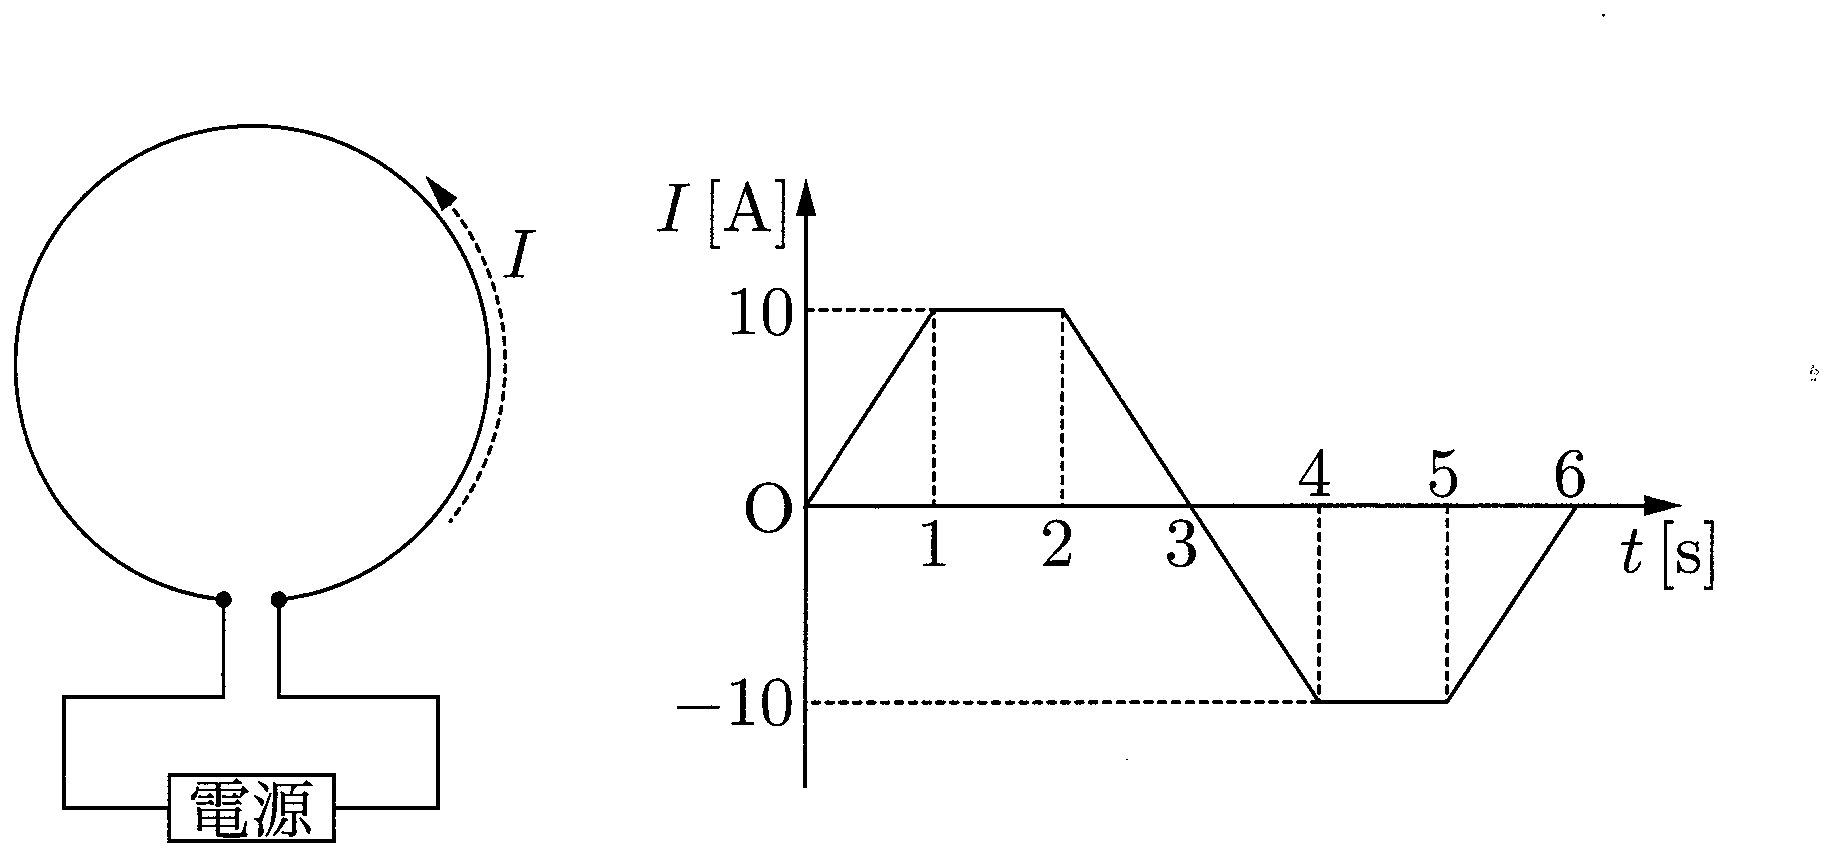
\includegraphics[keepaspectratio,width=100mm]{fig/n31_p112_zu.png}\end{center}

\Mon[\Sitei]{コイルを含む直流回路の過渡現象}

\hspace{1zw}下図のように内部抵抗の無視できる起電力$E\U{V}$の電池$\mathrm{E}$，抵抗値が$R\U{\Omega}$の電気抵抗$\mathrm{R}$，自己インダクタンスが$L\U{H}$のコイル$\mathrm{L}$，スイッチ$\mathrm{S}$を組み合わせて回路を作る．今，時刻$t=0$にスイッチ$\mathrm{S}$を閉じたとき，回路を流れる電流$I\U{A}$が時刻$t$に対して下図のように変化した．これについて以下の設問に答えよ．
\begin{center}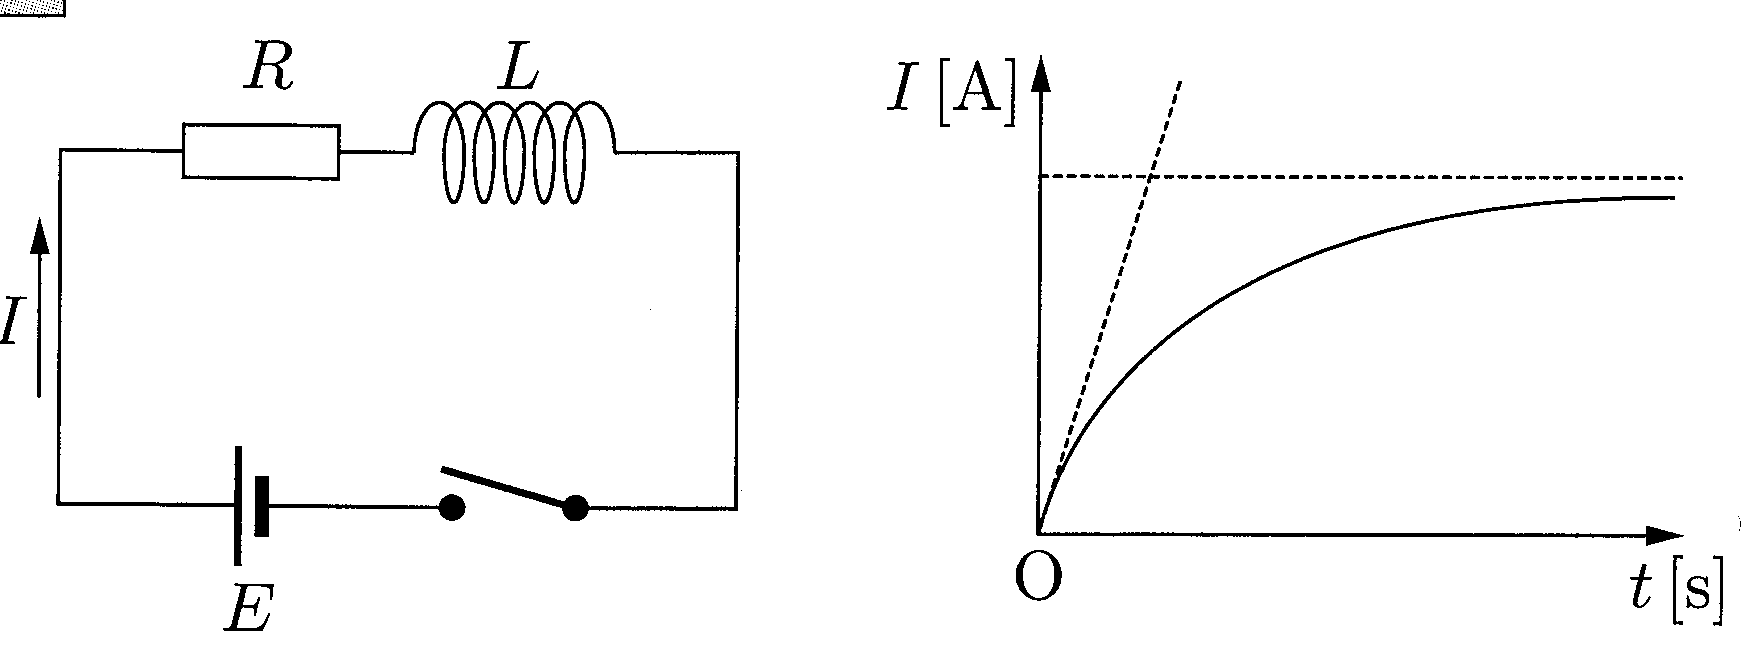
\includegraphics[keepaspectratio,width=100mm]{fig/n31_p113_zu.png}\end{center}
\begin{komon}
\ko{1} 時刻$t=0$における$I$-$t$グラフの接線の傾きを求めよ．
\ko{2} 十分時間が経ったとき，回路を流れる一定電流の大きさを求めよ．
\end{komon}

\Mon[\Sitei]{LC電気振動}

\begin{zuright}{50mm}
\hspace{1zw}内部抵抗の無視できる起電力$E\U{V}$の電池$\mathrm{E}$，電気容量$C\U{F}$のコンデンサー$\mathrm{C}$，自己インダクタンス$L\U{H}$のコイル$\mathrm{L}$，抵抗値$R\U{\Omega}$の電気抵抗$\mathrm{R}$，スイッチ$\mathrm{S}$を右図のように接続した．はじめ$\mathrm{S}$は開いており，$\mathrm{C}$には電荷が蓄えられていない．以下の設問に答えよ．
\par
\hspace{1zw}まず$\mathrm{S}$を閉じ，十分時間を経過させた．
\begin{komon}
\ko{1} 定常状態において，コイルを下向きに流れる電流$I_0$を求めよ．
\end{komon}
\zusep
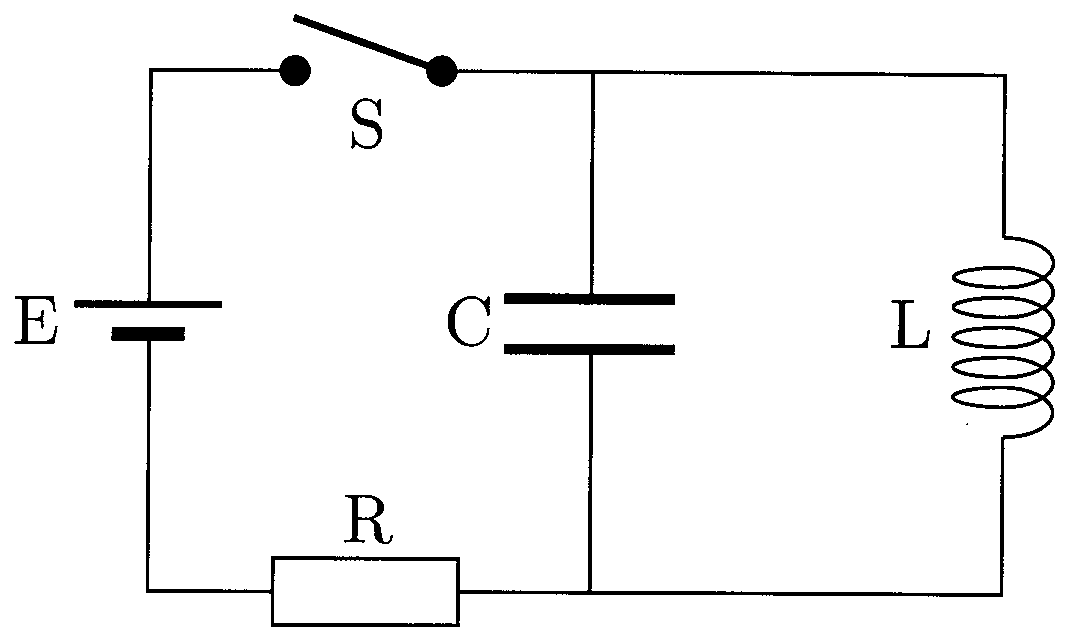
\includegraphics[keepaspectratio,width=48mm]{fig/n31_p114_zu.png}
\end{zuright}
\hspace{1zw}続いて$\mathrm{S}$を開いた．$\mathrm{S}$を開いた時刻を$t=0$とする．
\begin{komon}
\ko{2} 時刻$t$において，$\mathrm{C}$の上側極板に蓄えられる電気量を$Q(t)\U{C}$，図のLC回路部分に時計回りに流れる電流を$I(t)\U{A}$とする．$Q(t)$と$I(t)$の間に成り立つ微分関係を示せ．
\ko{3} キルヒホッフの第二法則を用いて時刻$t$において回路に成り立つ関係式を示せ．
\ko{4} (2)(3)を元に，回路の電気振動の周波数$f$および周期$T$を求めよ．
\ko{5} $Q(t)$および$I(t)$を求めよ．
\ko{6} 時刻$t$においてコイル$\mathrm{L}$，コンデンサー$\mathrm{C}$に蓄えられるエネルギー$E_{\mathrm{L}}(t)$，$E_{\mathrm{C}}(t)$を求めよ．
\end{komon}

\Mon{交流発電機}

\begin{zuright}{58mm}
\hspace{1zw}面積$S\U{m^2}$のひと巻きコイルを，磁束密度$B\U{Wb/m^2}$の一様な磁場中で図1の矢印の向きに角速度$\omega\U{rad/s}$で回すと，端子$\mathrm{PQ}$間に交流電圧が発生する．時刻$t=0$において，コイルは磁場に対して図2のように垂直になっていた．これについて以下の設問に答えよ．
\begin{komon}
\ko{1} 時刻$t$においてコイルを貫く磁束$\varPhi(t)\U{Wb}$を求めよ．
\ko{2} 時刻$t$において$\mathrm{P}$に対する$\mathrm{Q}$の電位$V(t)\U{V}$を求めよ．
\end{komon}
\zusep
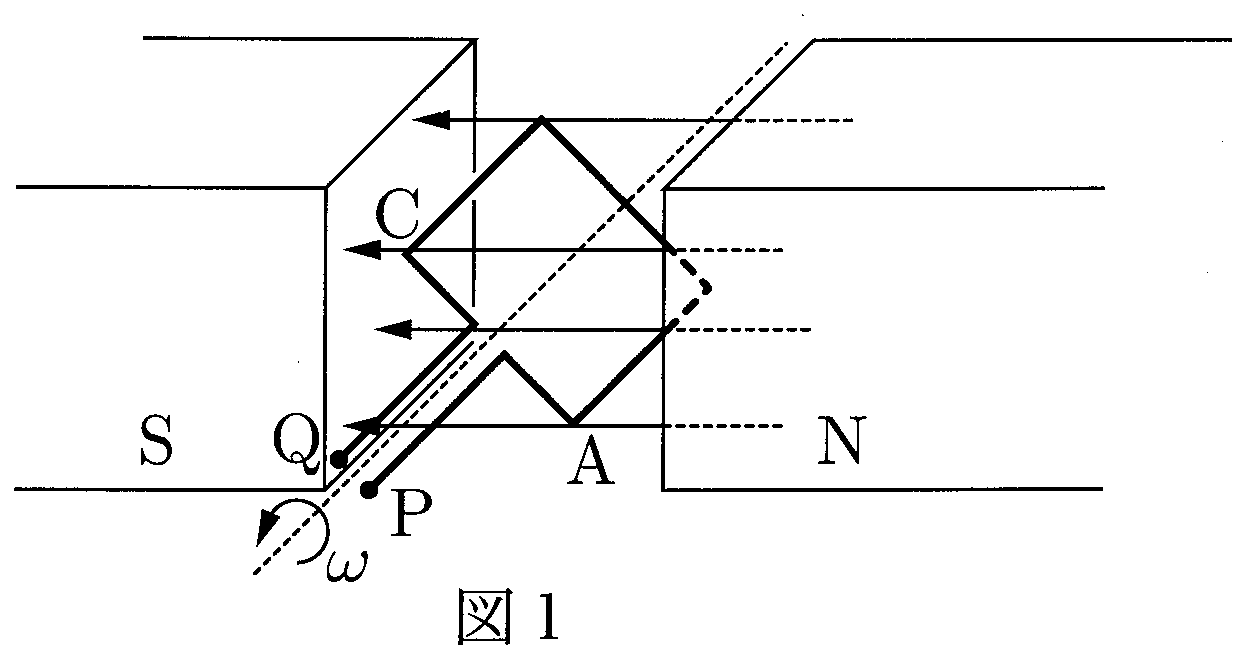
\includegraphics[keepaspectratio,width=56mm]{fig/n31_p115_zu1.png}\\[2mm]
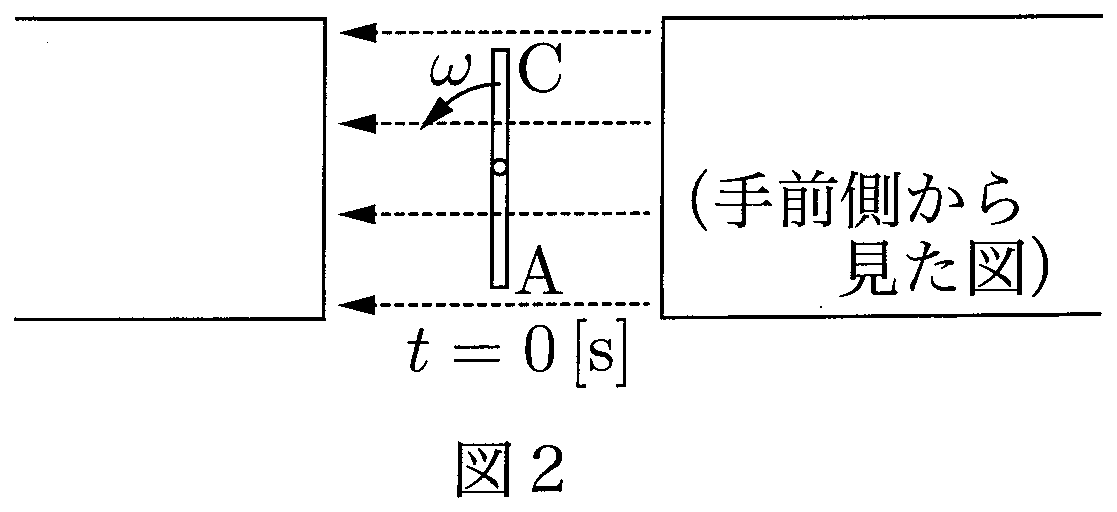
\includegraphics[keepaspectratio,width=52mm]{fig/n31_p115_zu2.png}
\end{zuright}

\Mon{力率}

\hspace{1zw}今，ある素子$\mathrm{A}$に対して$V(t)=V_0\sin\omega t\U{V}$で表される交流電圧をかけたところ，この素子$\mathrm{A}$には$I(t)=I_0\sin(\omega t+\varphi)\U{A}$で表される交流電流が流れた．これについて以下の設問に答えよ．
\begin{komon}
\ko{1} この素子の時刻$t$における消費電力$P(t)$を求めよ．
\ko{2} 消費電力の時間平均$\overline{P}$を求めよ．
\end{komon}

\Mon[\Sitei]{素子にかかる交流電圧と流れる交流電流の関係}

\hspace{1zw}図1〜3はそれぞれ，交流電源に抵抗値$R\U{\Omega}$の抵抗体$\mathrm{R}$，電気容量$C\U{F}$のコンデンサー$\mathrm{C}$，自己インダクタンス$L\U{H}$のコイル$\mathrm{L}$を接続したものである．交流電源の$-$に対する$+$の電圧が$V(t)=V_0\sin\omega t\U{V}$，グラフ(a)で示される時間変化をしているとき，次の各量について，その時間変動を表すグラフを選び，その時間変化を関数として示し，さらにその量の実効値を示せ．ただし，関数は$\sin\bigl(\omega t+\frac{\pi}{2}\bigr)$といった位相のずれの形で示しても，または$\cos\omega t$などと書き換えて示してもいずれでもよい．また，電流については図の矢印の向きを正として答えよ．
\begin{komon}
\ko{1} 図1において，抵抗を流れる電流$I_{\mathrm{R}}(t)$
\ko{2} 図1において，抵抗で消費されている電力$P_{\mathrm{R}}(t)$
\ko{3} 図2において，コンデンサーの上側極板に蓄えられている電荷$Q_{\mathrm{C}}(t)$（この(3)のみ実効値は示さなくてよい）
\ko{4} 図2において，コンデンサーを通じて流れる電流$I_{\mathrm{C}}(t)$
\ko{5} 図2において，コンデンサーで消費されている電力$P_{\mathrm{C}}(t)$
\ko{6} 図3において，コイルの自己誘導起電力$V_{\mathrm{L}}(t)$（ただし図で示した向きの電流を流す電圧の向きを正として答えよ）
\ko{7} 図3において，コイルを通じて流れる電流$I_{\mathrm{L}}(t)$
\ko{8} 図3において，コイルで消費されている電力$P_{\mathrm{L}}(t)$
\end{komon}
\begin{center}
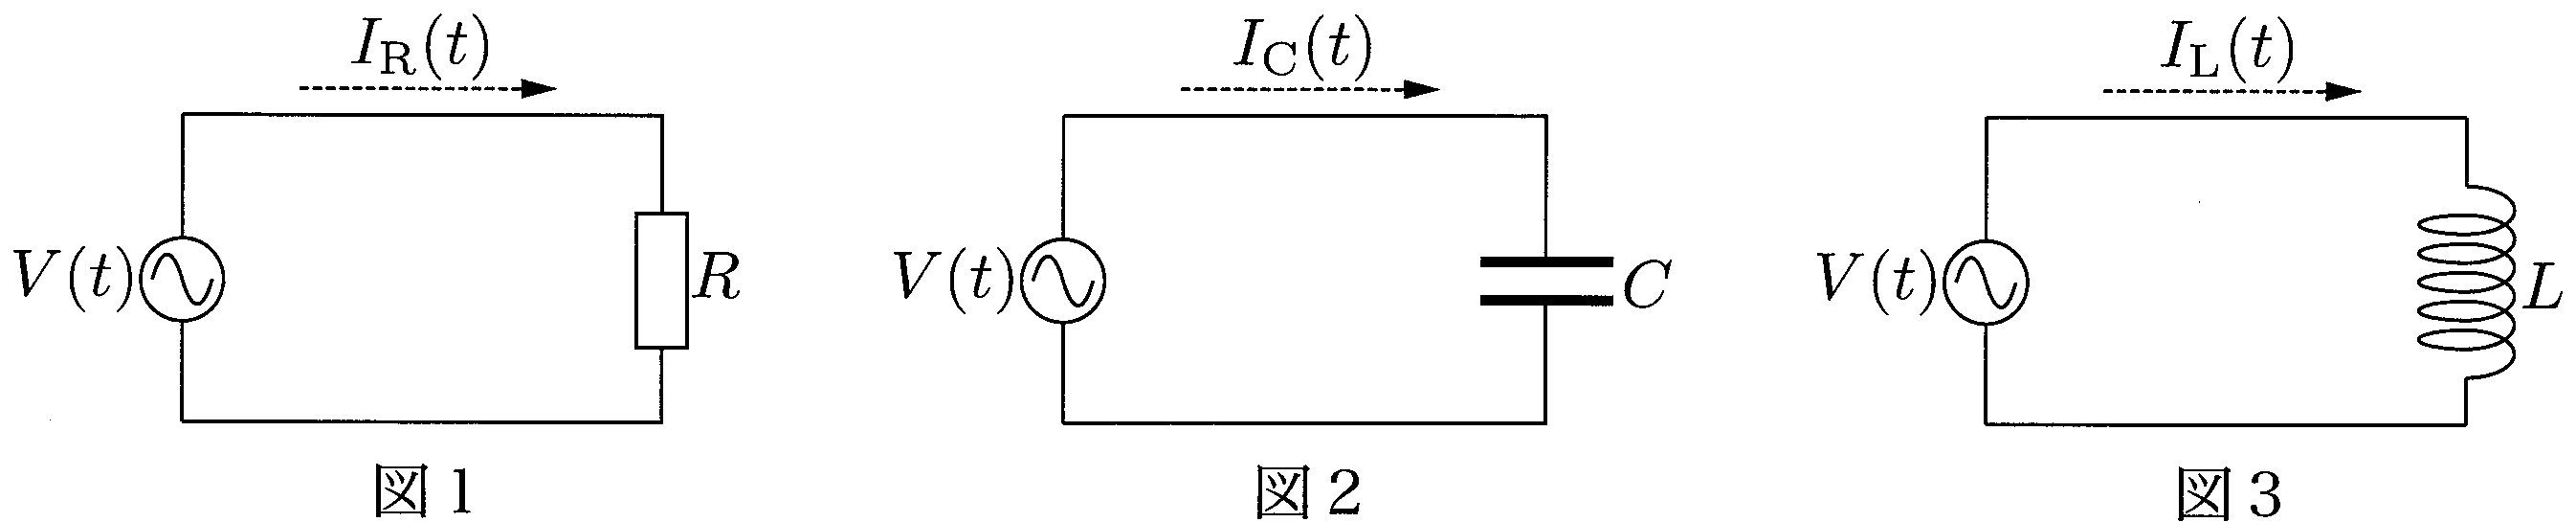
\includegraphics[keepaspectratio,width=130mm]{fig/n31_p117_zu.png}\\[3mm]
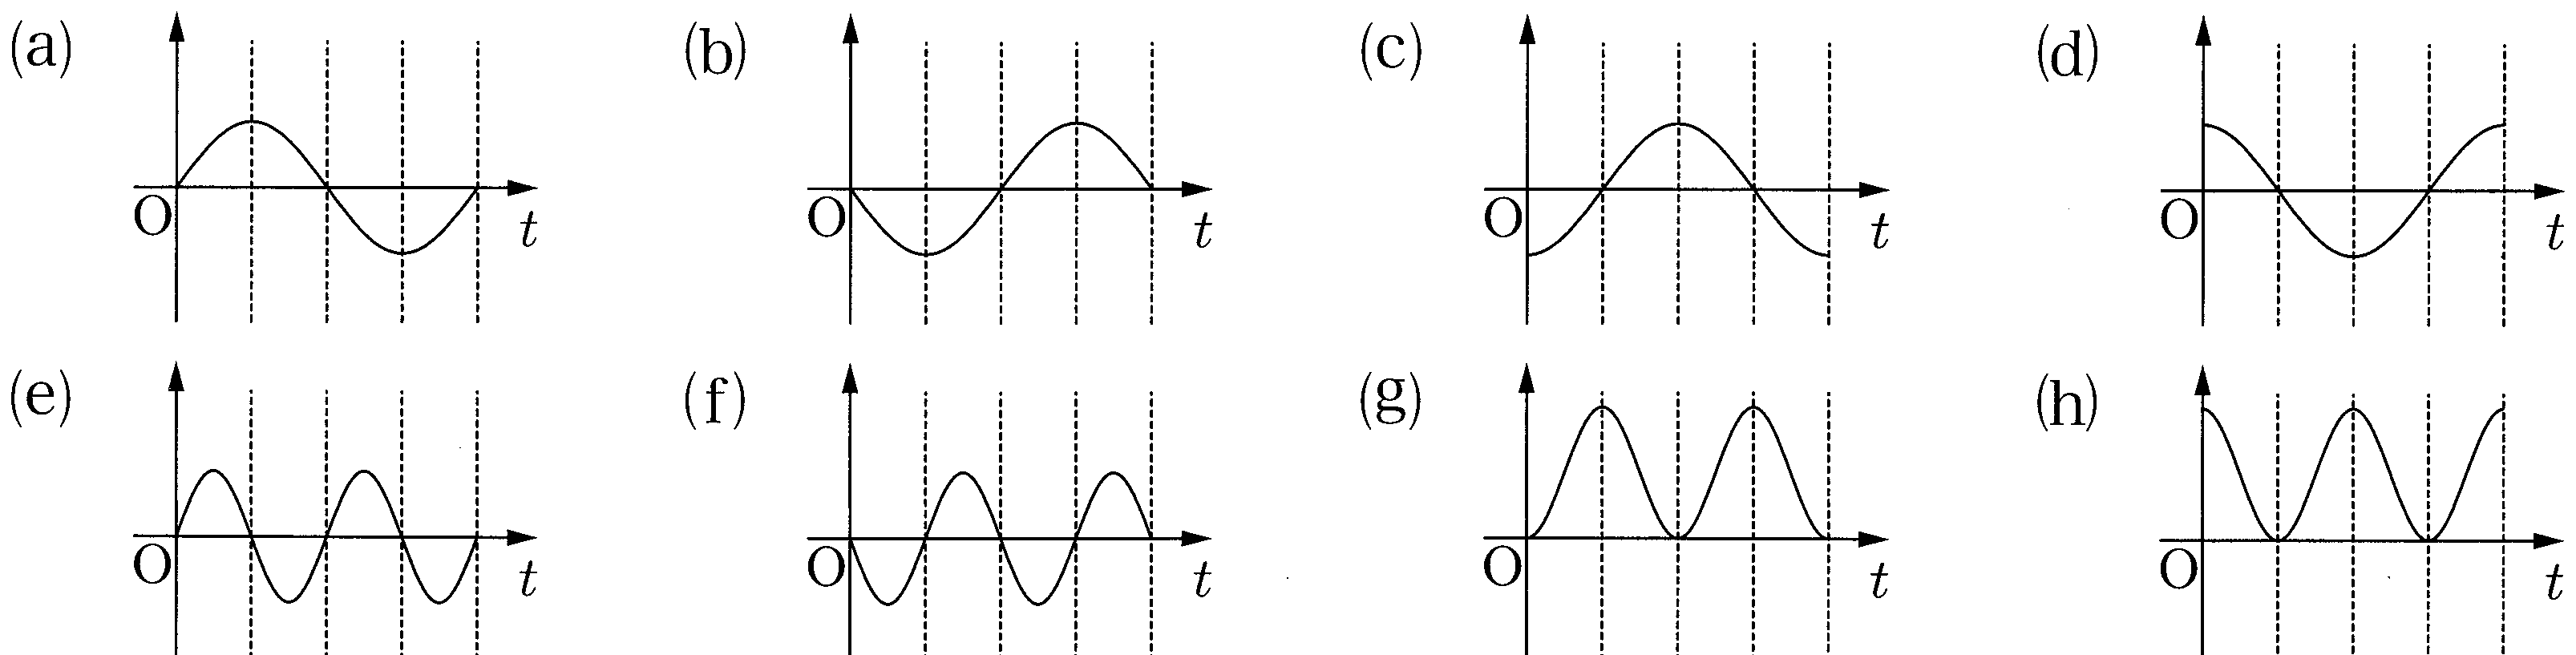
\includegraphics[keepaspectratio,width=150mm]{fig/n31_p117_graph.png}
\end{center}

\filbreak
\Rank{C問題}

\Mon{中心点のずれたLC電気振動}

\begin{zuright}{56mm}
\hspace{1zw}内部抵抗の無視できる起電力$E\U{V}$の電池$\mathrm{E}$，電気容量がいずれも$C\U{F}$のコンデンサー$\mathrm{C}_1$，$\mathrm{C}_2$，自己インダクタンス$L\U{H}$のコイル$\mathrm{L}$，スイッチ$\mathrm{S}_1$，$\mathrm{S}_2$を右図のように接続した．はじめ$\mathrm{S}_1$，$\mathrm{S}_2$はいずれも開いており，$\mathrm{C}_1$，$\mathrm{C}_2$のいずれにも電荷が蓄えられていない．これについて以下の設問に答えよ．
\zusep
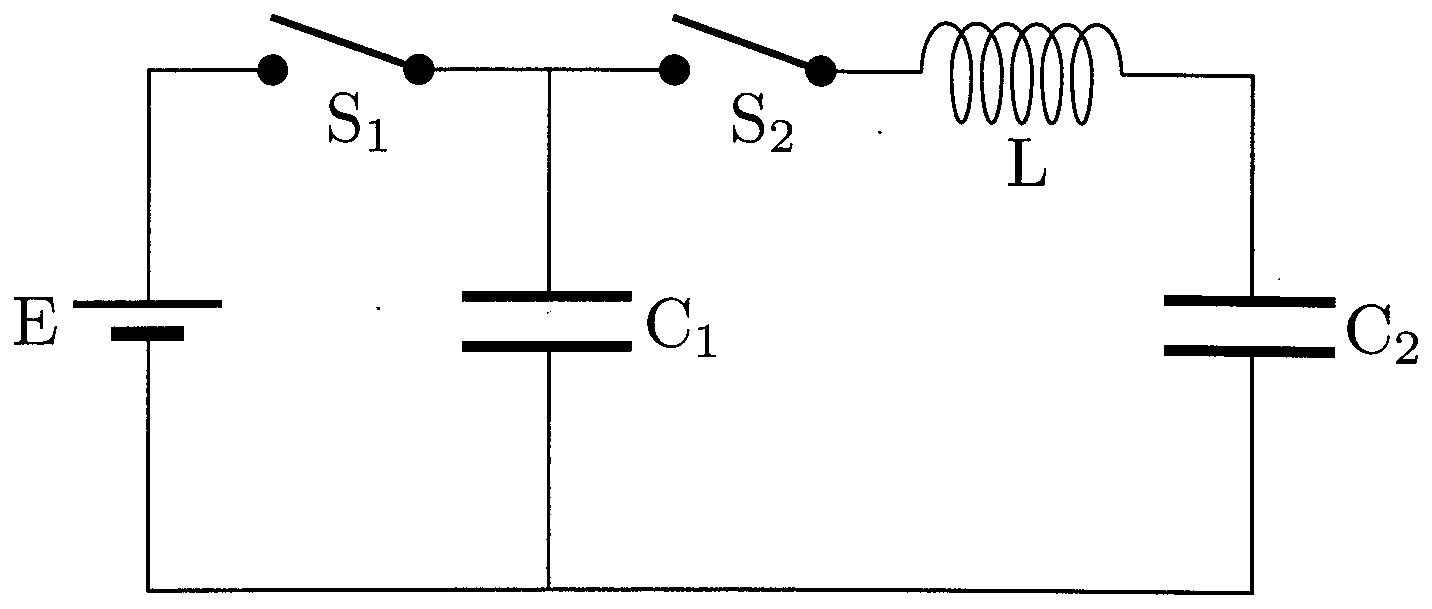
\includegraphics[keepaspectratio,width=54mm]{fig/n31_p118_zu.png}
\end{zuright}
\begin{komon}
\ko{1} まず，スイッチ$\mathrm{S}_1$のみを閉じて十分な時間を経過させた．このとき，コンデンサー$\mathrm{C}_1$の上側極板に蓄えられる電気量を求めよ．
\ko{2} 続いてスイッチ$\mathrm{S}_1$を開き，時刻$t=0$にスイッチ$\mathrm{S}_2$を閉じた．時刻$t$においてコンデンサー$\mathrm{C}_1$，$\mathrm{C}_2$の上側極板に蓄えられている電気量を$Q_1(t)$，$Q_2(t)\U{C}$，右側のLC回路部に時計回りに流れる電流を$I(t)\U{A}$とおく．このとき，まず電荷保存則より$Q_1(t)$，$Q_2(t)$の間に成り立つ関係式を示せ．
\ko{3} 次に，電荷と電流の関係より$Q_1(t)$，$Q_2(t)$，$I(t)$の間に成り立つ関係式を示せ．
\ko{4} キルヒホッフの第二法則を用いて時刻$t$において回路に成り立つ関係式を示せ．
\ko{5} この回路で起こるLC電気振動の周期を求めよ．
\ko{6} コンデンサー$\mathrm{C}_1$の上側極板の電気量$Q_1(t)$はどの範囲で振動するか．
\end{komon}

\Mon{素子にかかる交流電圧と流れる交流電流の関係}

\hspace{1zw}瞬時値が$I(t)=I_0\sin\omega t\U{A}$で表される交流電流が，抵抗値$R\U{\Omega}$の抵抗体，自己インダクタンス$L\U{H}$のコイル，電気容量$C\U{F}$のコンデンサーにそれぞれ流れているとき，各回路素子にかかっている電圧の瞬時値$V_{\mathrm{R}}(t)$，$V_{\mathrm{L}}(t)$，$V_{\mathrm{C}}(t)\U{V}$を求めよ．ただし，電流の流れる向きに沿って電圧降下が起こっている場合を正として答えよ．

\newpage

%%%%%%%%%%%%%%%%%%%%  解答  %%%%%%%%%%%%%%%%%%%%
\KaiTitle{第31回　回路の過渡現象・電気振動と交流の基礎}
\setlength{\columnseprule}{0.4pt}
\begin{multicols}{2}
\raggedcolumns

\Rank{A問題}
\MonN{111}{基本公式の確認}\par\nopagebreak
\begin{sisin}
単に「消費電力」といった場合は，平均値を考えている点に注意．また，電流・電圧の実効値とは瞬時値の最大値の$\dfrac{1}{\sqrt{2}}$倍と定義されている．これにより，交流においても消費電力が$\overline{P}=V_{\mathrm{e}}I_{\mathrm{e}}$と表せ，直流と同様になるのである．

実効値と瞬時値をはっきりと区別するためにも，瞬時値は$V(t)$，$I(t)$など，実効値は$V_{\mathrm{e}}$，$I_{\mathrm{e}}$などとし，瞬時値の最大値は$V_0$，$I_0$などとして書き分けるとよい．これら三つをごっちゃにしないようにせよ．誘導リアクタンス，容量リアクタンスの単位が$\U{\Omega}$であることを忘れないように．
\end{sisin}
\KaiHead
\begin{komon}
\ko{1} \[V_0=\sqrt{2}\cdot V_{\mathrm{e}}=100\sqrt{2}\fallingdotseq 141\U{V}\Ans\]
\ko{2} \[\begin{aligned}\overline{P}&=V_{\mathrm{e}}I_{\mathrm{e}}=\frac{V_0}{\sqrt{2}}\cdot\frac{I_0}{\sqrt{2}}\\&=\frac{100}{\sqrt{2}}\cdot\frac{1}{\sqrt{2}}=50\U{W}\Ans\end{aligned}\]
       （$\overline{P}=\dfrac{1}{2}V_0I_0=50\U{W}$としてもよい．）
\ko{3} \[\begin{aligned}X_L&=\omega L=2\pi fL=2\cdot 3.14\cdot 100\cdot 10\\&=6.28\times 10^3\U{\Omega}\Ans\end{aligned}\]
\ko{4} % 原本は分母を 100×10^{-6} と書いていた（問題文は 10 μF．答の値は 10 μF で正しい）．
       \[\begin{aligned}X_C&=\frac{1}{\omega C}=\frac{1}{2\pi fC}\\&=\frac{1}{2\cdot 3.14\cdot 100\cdot(10\times 10^{-6})}\\&\fallingdotseq 1.59\times 10^2\U{\Omega}\Ans\end{aligned}\]
\end{komon}

\Rank{B問題}
\MonN{112}{自己誘導起電力}\par\nopagebreak
\begin{sisin}
電流変化のグラフから誘導起電力を求めさせる本問のようなタイプの問題では，元ある電流が流れている向きが誘導電流にとっても正の向きになることに注意する．この向きの電流を流そうとする起電力の向きを正として，誘導起電力が$-L\dfrac{dI}{dt}$と表されることになる．問題で誘導起電力の向きが指定されているときには必ず自分で考えた向きと合致しているかどうかチェックしなければならない．

自己誘導については元ある電流が増加するときに誘導起電力は負の向きに，減少するときに正の向きに発生するので，検算に利用することができる．
\end{sisin}
\KaiHead
反時計回りに流れる電流の向きが正であるので，発生する誘導起電力は，
\[V=-L\frac{dI}{dt}=-0.010\frac{dI}{dt}\]
と表される．ここで図2より，電流の時間変化率は，
\[\frac{dI}{dt}=\left\{\begin{aligned}
  &+10\U{A/s}\quad(0<t<1)\\
  &\ 0\U{A/s}\quad(1<t<2)\\
  &-10\U{A/s}\quad(2<t<4)\\
  &\ 0\U{A/s}\quad(4<t<5)\\
  &+10\U{A/s}\quad(5<t<6)
\end{aligned}\right.\]
であるから，求めるグラフは次図のようになる．\Ans
\begin{center}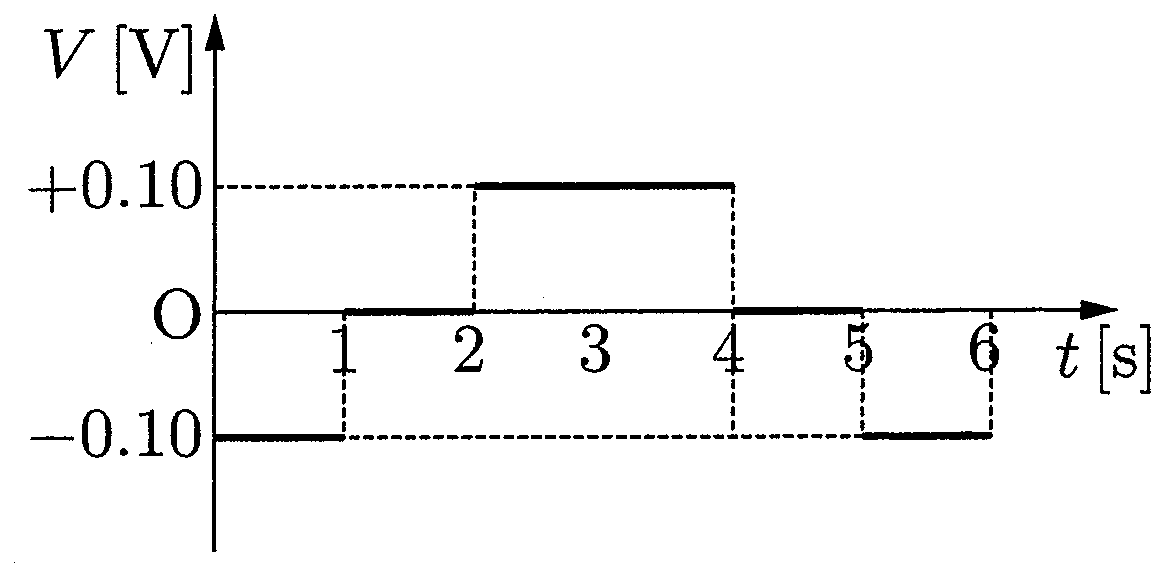
\includegraphics[keepaspectratio,width=52mm]{fig/n31_a112_graph.png}\end{center}

\MonN[\Sitei]{113}{コイルを含む直流回路の過渡現象}\par\nopagebreak
\begin{sisin}
コイルやコンデンサーなどを含む直流回路について，電流の時間変化を問うタイプの問題では，まず回路についてキルヒホッフの第二法則を用いて立式し，これを解釈するというのが基本的な流れである．電流の時間変化率$\dfrac{dI}{dt}$について解き，最初の$t=0$，$I=0$の状態からどのように電流$I$が変化するのかを考えよう（例題35）．

直流回路にコイルが含まれている場合，「\MARU{1}スイッチを入れた直後はすぐには電流が変わらない（電流$0$のコイルは切れた導線のようにふるまう）．\MARU{2}十分時間が経つとコイルは抵抗値$0$の導線のようにふるまい，電流が変化しなくなる．」という知識を利用して解く方法もある（31.1）．
\end{sisin}
\KaiHead
時刻$t$における電流を$I(t)$とし，回路にキルヒホッフの第二法則を用いて立式すると，
\[E+\Bigl(-L\frac{dI}{dt}\Bigr)=RI\qquad\cdots\text{\MARU{1}}\]
となる．
\begin{center}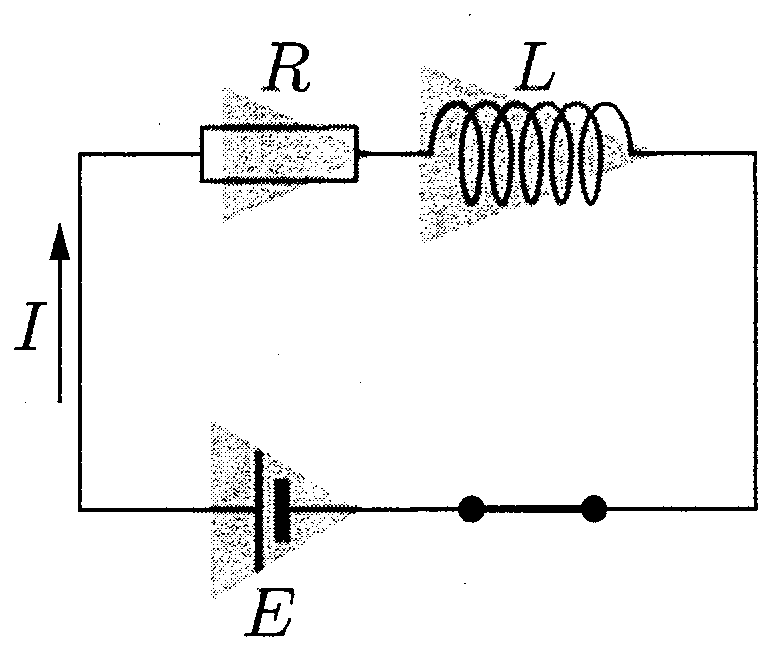
\includegraphics[keepaspectratio,width=36mm]{fig/n31_a113_zu.png}\end{center}
\begin{komon}
\ko{1} \MARU{1}式より，$\dfrac{dI}{dt}=\dfrac{E-RI}{L}$．最初の$t=0$では$I=0$であるから，代入すると
       \[\frac{dI}{dt}\Big|_{t=0}=\frac{E}{L}\U{A/s}\Ans\]
       これが$I$-$t$グラフの$t=0$における接線の傾きである．
\ko{2} $t=0$のときは$\dfrac{dI}{dt}=\dfrac{E}{L}>0$であるから徐々に電流$I(t)$が$0$から増加していくことになるが，$I(t)$が増加すると$\dfrac{dI}{dt}$が減っていく．すなわち，電流の増加率が減ることになる．$\dfrac{dI}{dt}=0$まで減少してしまうとそれ以上電流は増加しなくなるため，$I(t)$は一定の大きさとなる．よって，十分時間が経過したときの電流は，\MARU{1}式にて$\dfrac{dI}{dt}=0$とおいて$E=RI$より，
       \[I=\frac{E}{R}\U{A}\Ans\]
\end{komon}
\begin{bsHosoku}{参考}
上の(2)の説明は直感的なもので，厳密には微分方程式を解く必要がある．\MARU{1}を$\dfrac{dI}{I-\frac{E}{R}}=-\dfrac{R}{L}dt$と変形して積分し，$t=0$で$I=0$を用いると
\[I(t)=\frac{E}{R}\Bigl(1-e^{-\frac{R}{L}t}\Bigr)\]
となり，$t\to\infty$で$\dfrac{E}{R}$に近づく．
\begin{center}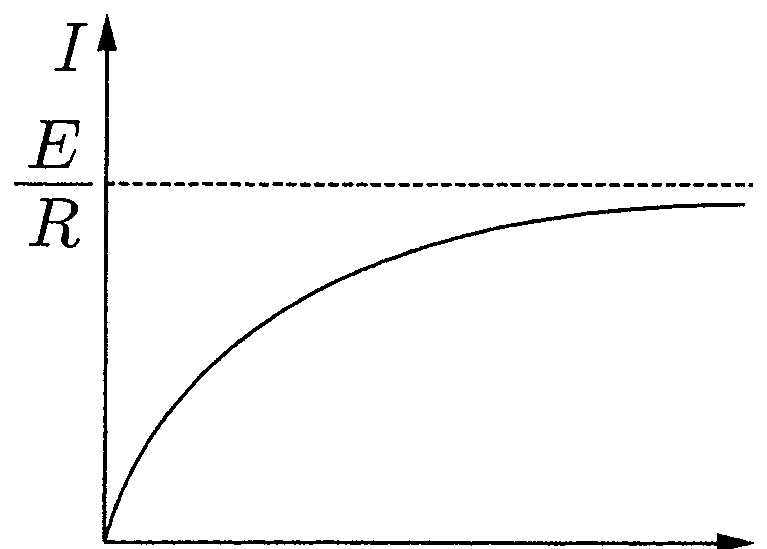
\includegraphics[keepaspectratio,width=36mm]{fig/n31_a113_graph.png}\end{center}
\end{bsHosoku}

\MonN[\Sitei]{114}{LC電気振動}\par\nopagebreak
\begin{sisin}
電気振動の振動数を求める一般的な解法を覚えておくこと．
\MARU{1}\ 初期状態（コイルに流れる電流，コンデンサーの電荷）を調べておく．
\MARU{2}\ 時刻$t$のコンデンサーの帯電量およびコイルを流れる電流を$\pm Q(t)$，$I(t)$とおく（向きは自由に取ってよい）．
\MARU{3}\ 電流と電荷の間に成り立つ微分関係を決定する．
\MARU{4}\ キルヒホッフの第二法則を立てる．
\MARU{5}\ 二つの式から$I(t)$を消去して$Q(t)$の微分方程式を作る．
\MARU{6}\ 微分方程式から角周波数を求め，周波数・周期を求める．
\MARU{7}\ 初期条件を当てはめて$Q(t)$，$I(t)$を得る．

電気振動ではもう一つ，エネルギー保存則から攻める方法もある（31.2）．固有周波数を求めるなら前者，最大値を求めるなら後者が便利である．
\end{sisin}
\KaiHead
\begin{komon}
\ko{1} Sを閉じて十分時間がたつと，コンデンサーには電流が流れ込まなくなり，コイルを流れる電流は一定値になる．よって，コイルには自己誘導起電力が発生せず，コンデンサーの帯電量は$0$である（次図参照）．
       \begin{center}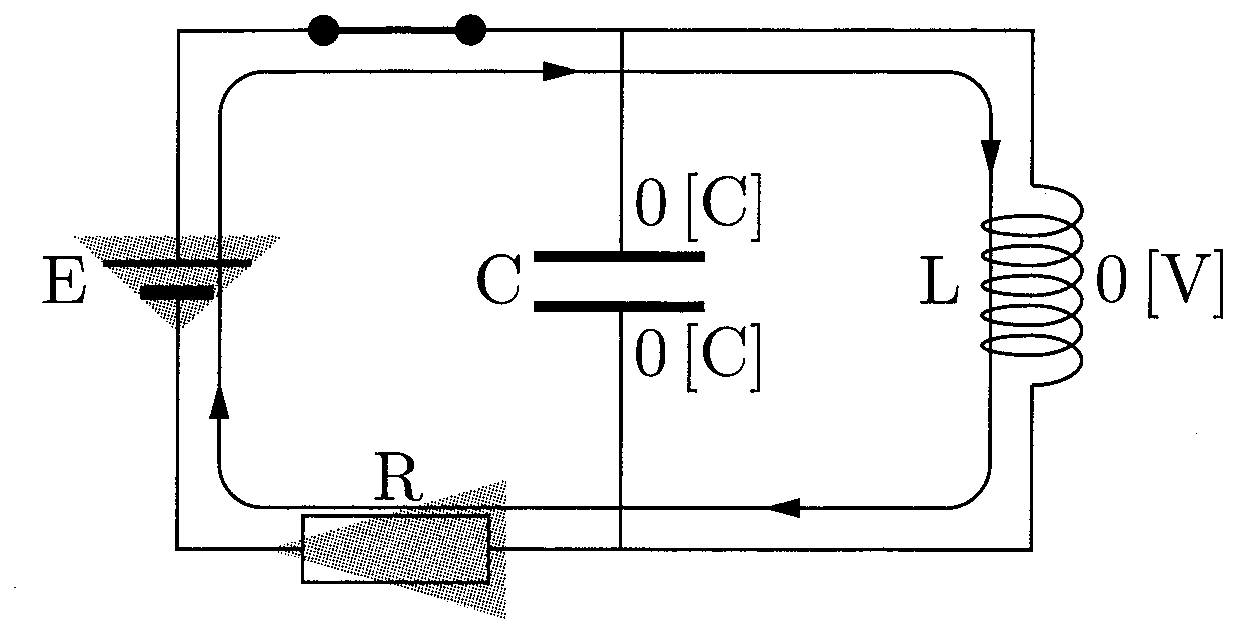
\includegraphics[keepaspectratio,width=50mm]{fig/n31_a114_zu1.png}\end{center}
       このときのキルヒホッフの第二法則より$E=RI_0$．ゆえに，
       \[I_0=\frac{E}{R}\U{A}\Ans\]
       \begin{chuu}
       (1)の場合は回路に抵抗が含まれているため十分時間が経つと電流が一定になるが，(2)以降の抵抗を含まない回路では，十分時間が経過しても電流は一定にならず，電気振動する．
       \end{chuu}
\ko{2} スイッチSを開くと，コイルから抵抗に流れ込んでいた電流がコンデンサーへと流れ込むようになる．この回路はL，CのみからなるLC振動回路であるから電気振動が発生する．
       \begin{center}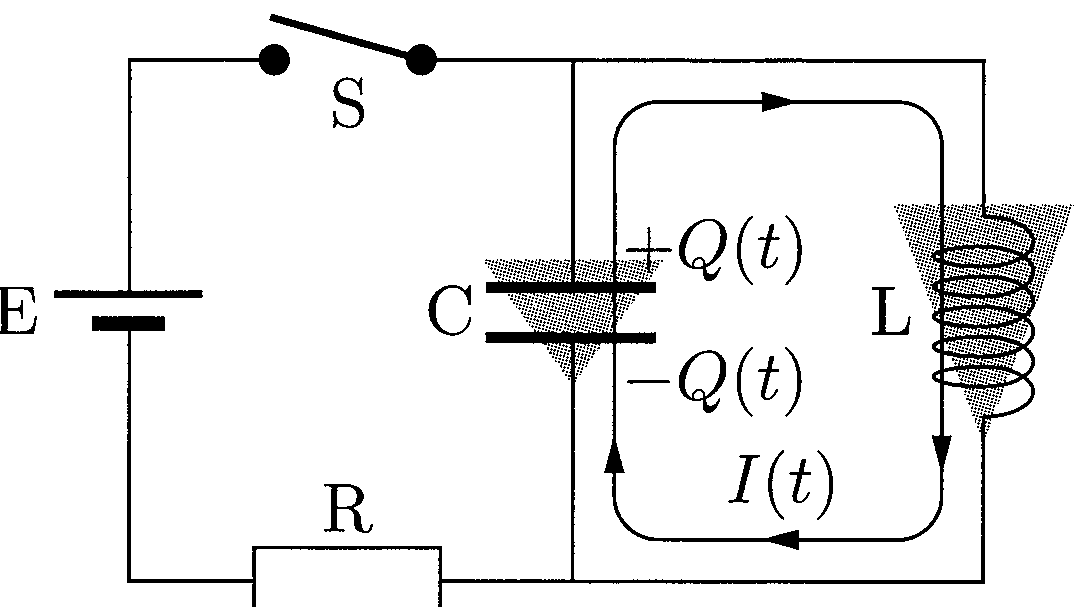
\includegraphics[keepaspectratio,width=50mm]{fig/n31_a114_zu2.png}\end{center}
       このとき，電流$I(t)$の流入によりコンデンサーの下側極板の電荷$-Q(t)$が増加するので，$\dfrac{d\{-Q(t)\}}{dt}=I(t)$．整理して，
       \[I(t)=-\frac{dQ(t)}{dt}\Ans\]
\ko{3} 上側極板の電荷が$Q(t)$であることに注意してキルヒホッフの第二法則より立式すると，
       \[-L\frac{dI(t)}{dt}=\frac{-Q(t)}{C}\Ans\]
\ko{4} (2)の両辺を$t$で微分して(3)に代入し，整理すると，
       \[\frac{d^2Q(t)}{dt^2}=-\frac{1}{LC}Q(t)\]
       である．これは，$Q(t)$が角周波数$\omega=\dfrac{1}{\sqrt{LC}}$で電気振動することを意味する．よって，
       \[f=\frac{\omega}{2\pi}=\frac{1}{2\pi\sqrt{LC}}\U{Hz}\Ans\]
       \[T=\frac{1}{f}=2\pi\sqrt{LC}\U{s}\Ans\]
       \begin{chuu}
       角周波数の取り方は単振動の場合と全く同様である．単振動の場合は運動方程式を$\dfrac{d^2x}{dt^2}=-\omega^2(x-x_0)$の形に整理して振動中心$x_0$および角振動数$\omega$を得た．本問でも$\dfrac{d^2Q}{dt^2}=-(\text{定数})\times\{Q-\text{定数}\}$の形に変形し，最初の定数部分を$\omega^2$と置けばよい．
       \end{chuu}
\ko{5} $t=0$のとき，$Q(0)=0$，$I(0)=I_0>0$である．(2)より$\dfrac{dQ}{dt}=-I(0)<0$であり，$Q(t)$は減少していく．$Q(t)$の取る最大値を$Q_0$としておくと，$Q(t)$の時間変動は次のようなグラフになる．
       \begin{center}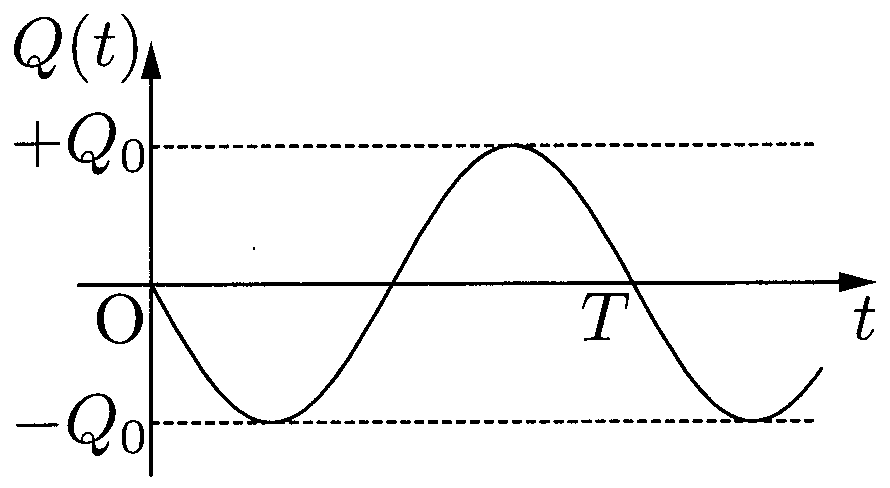
\includegraphics[keepaspectratio,width=44mm]{fig/n31_a114_graph.png}\end{center}
       よって$Q(t)=-Q_0\sin\omega t$．(2)より$I(t)=\omega Q_0\cos\omega t$であるが，$I(0)=I_0$より$\omega Q_0=\dfrac{E}{R}$．これを解いて，$Q_0=\dfrac{E}{R}\sqrt{LC}$．以上より，
       \[\left\{\begin{aligned}
         Q(t)&=-\frac{E}{R}\sqrt{LC}\sin\frac{t}{\sqrt{LC}}\U{C}\\
         I(t)&=\frac{E}{R}\cos\frac{t}{\sqrt{LC}}\U{A}
       \end{aligned}\right.\]
       \hspace*{\fill}$\cdots$(答)
       \begin{bekkai}
       エネルギー保存則$\dfrac{1}{2}L\{I(t)\}^2+\dfrac{\{Q(t)\}^2}{2C}=\dfrac{1}{2}LI_0^2$を使えば，電荷が最大のとき$I=0$なので$\dfrac{Q_0^2}{2C}=\dfrac{1}{2}LI_0^2$より$Q_0=I_0\sqrt{LC}=\dfrac{E}{R}\sqrt{LC}$が直ちに得られる．
       \end{bekkai}
\ko{6} \[\begin{aligned}
         E_{\mathrm{L}}(t)&=\frac{1}{2}L\{I(t)\}^2\\&=\frac{LE^2}{2R^2}\cos^2\frac{t}{\sqrt{LC}}\U{J}\\
         E_{\mathrm{C}}(t)&=\frac{\{Q(t)\}^2}{2C}\\&=\frac{LE^2}{2R^2}\sin^2\frac{t}{\sqrt{LC}}\U{J}
       \end{aligned}\]
       \hspace*{\fill}$\cdots$(答)
       和は$\dfrac{LE^2}{2R^2}$（一定）であり，エネルギー保存則が成り立っている．
\end{komon}

\MonN{115}{交流発電機}\par\nopagebreak
\begin{sisin}
コイル面に対して斜めに磁場がかかっている場合にコイルを貫く磁束を計算する際には，磁場に対して垂直な面成分がどれだけあるのかを考えよ．
（磁束）$=$（磁束密度）$\times$（磁場に垂直な面成分）として求めるか，（磁束）$=$（面の面積）$\times$（面に垂直な磁束密度成分）として求めよう．

発生する誘導起電力については，コイルが最初の状態にあるときに磁石のつくる磁場と同じ向きの磁場を生じる電流の向きを正とすれば，ファラデーの電磁誘導の法則$e=-\dfrac{d\varPhi}{dt}$が利用できる．
\end{sisin}
\KaiHead
\begin{komon}
\ko{1} 時刻$t$において，コイルは次図のように最初の状態から角度$\omega t$だけ傾いている．
       \begin{center}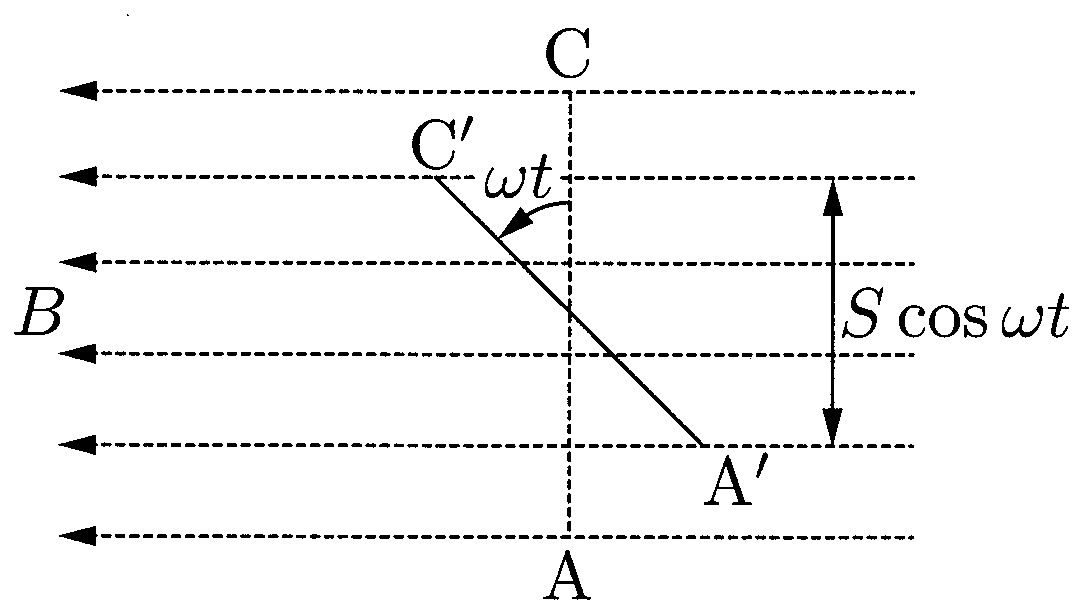
\includegraphics[keepaspectratio,width=46mm]{fig/n31_a115_zu1.png}\end{center}
       よって，磁束密度に対して垂直な面成分は$S\cos\omega t$であるから，
       \[\varPhi(t)=BS\cos\omega t\U{Wb}\Ans\]
\ko{2} コイルが最初の状態にあるときに左向きに磁場を発生させるには，コイル内を$\mathrm{Q}\to\mathrm{C}\to\mathrm{A}\to\mathrm{P}$の向きに電流が流れればよく，これが電流の正の向きとなる．このように電流がコイル内を流れたとき$\mathrm{P}$の方が電位が高くなるので，発生する誘導起電力$e(t)=-\dfrac{d\varPhi}{dt}$は$\mathrm{P}$が高電位の向きを正としている．求めるのは$\mathrm{P}$に対する$\mathrm{Q}$の電位であるから，
       \[\begin{aligned}V(t)&=-e(t)=\frac{d\varPhi}{dt}\\&=-\omega BS\sin\omega t\U{V}\Ans\end{aligned}\]
       \begin{center}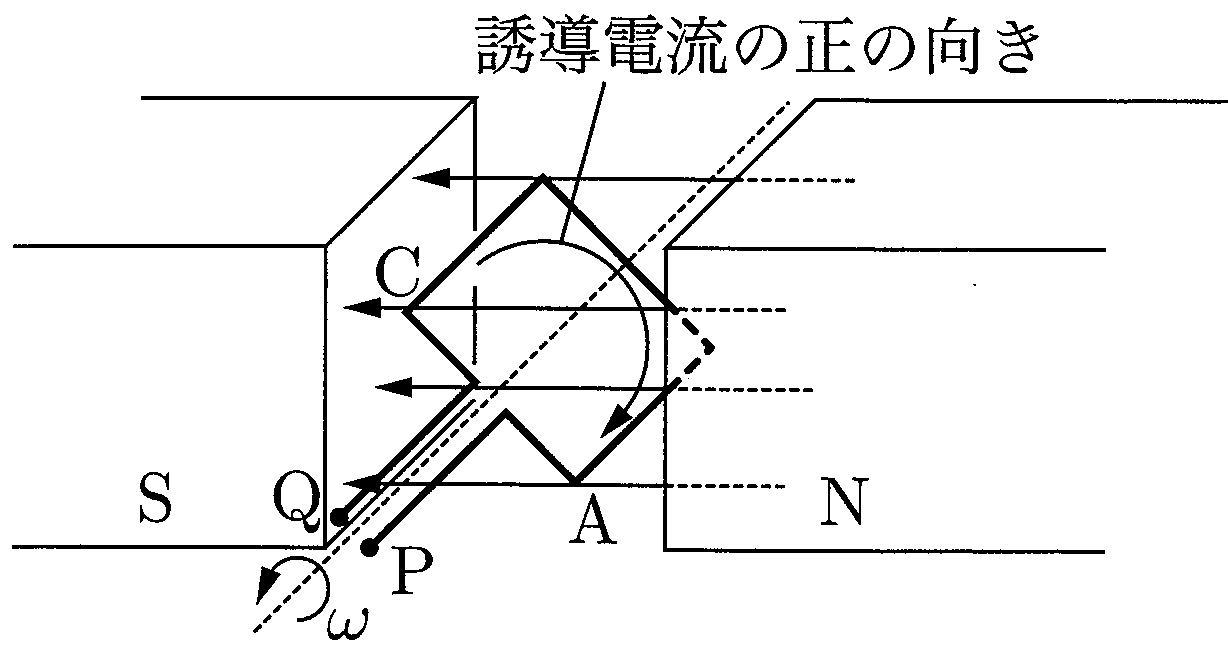
\includegraphics[keepaspectratio,width=52mm]{fig/n31_a115_zu2.png}\end{center}
\end{komon}

\MonN{116}{力率}\par\nopagebreak
\begin{sisin}
消費電力については，$P(t)$をグラフ化してみてその平均値がどうなるのかを考えればよいが，結果的に考えているのは$P$-$t$グラフの高さの平均値であり，一周期について$\overline{P}\cdot T=\displaystyle\int_0^TP(t)\,dt$を満たすような$\overline{P}$である（31.7）．
\end{sisin}
\KaiHead
\begin{komon}
\ko{1} \[\begin{aligned}P(t)&=V(t)I(t)\\&=V_0I_0\sin\omega t\sin(\omega t+\varphi)\U{W}\Ans\end{aligned}\]
\ko{2} 積和の公式$\sin\alpha\sin\beta=-\dfrac{1}{2}\{\cos(\alpha+\beta)-\cos(\alpha-\beta)\}$より
       \[P(t)=\frac{1}{2}V_0I_0\cos\varphi-\frac{1}{2}V_0I_0\cos(2\omega t+\varphi)\]
       第2項の時間平均は$0$であるから，
       \[\overline{P}=\frac{1}{2}V_0I_0\cos\varphi\U{W}\Ans\]
\end{komon}
\begin{bsHosoku}{参考}
一般に$\overline{P}=\dfrac{1}{T}\displaystyle\int_0^TP(t)\,dt$で与えられ，上式を代入して積分しても$\dfrac{1}{2}V_0I_0\cos\varphi$が得られる．
\end{bsHosoku}

\MonN[\Sitei]{117}{素子にかかる交流電圧と流れる交流電流の関係}\par\nopagebreak
\begin{sisin}
交流電流・電圧は，\MARU{1}瞬時値の最大値，\MARU{2}位相，という二つの要素によって記述することができる．あらかじめ，抵抗・コイル・コンデンサーの各素子について，\MARU{1}最大値の間に成り立つ関係式と，\MARU{2}位相の間に成り立つ関係，の二つを暗記しておけば（31.7 のまとめ枠），微積分を全く利用せずに，かけた電圧に対して流れる電流を求めることができる．

「位相が進む」「位相が遅れる」ということと実際の式の対応関係がごっちゃになりやすいのでまとめて整理しておくこと．例えば，「$I(t)$の位相は$V(t)$の位相に対して$\dfrac{\pi}{2}$だけ遅れる」とは，「$I(t)$の増減変化は，$V(t)$の増減変化に対して$\dfrac{1}{4}$周期だけ遅れて起こる」ということを意味する．数式的には，$V(t)$の位相部分が$\omega t+\alpha$であったのなら，$I(t)$の位相部分は$\omega t+\alpha-\dfrac{\pi}{2}$になる．

グラフとの対応関係も間違いやすいので注意せよ．「$I(t)$は$V(t)$に対して$\dfrac{1}{4}$周期だけ進んでいる」という場合，$I(t)$のグラフの凹凸は，$V(t)$のグラフの凹凸に対して{\gtfamily 左方向に}$\dfrac{1}{4}T$だけずれている．

消費電力の平均値が$\overline{P}=V_{\mathrm{e}}I_{\mathrm{e}}$で求められるのは抵抗の場合のみであり，一般には$\overline{P}=V_{\mathrm{e}}I_{\mathrm{e}}\cos\varphi$である（［116］）．
% 原本は「(→[30])」（旧回の番号）．
\end{sisin}
\KaiHead
各素子にかかっている電圧は$V(t)=V_0\sin\omega t$である．以下，実効値は添え字eで表す．
\begin{komon}
\ko{1} $V_0=RI_{\mathrm{R}0}$より$I_{\mathrm{R}0}=\dfrac{V_0}{R}$で，位相は電圧と同じなので
       \[I_{\mathrm{R}}(t)=\frac{V_0}{R}\sin\omega t\U{A},\quad I_{\mathrm{Re}}=\frac{\sqrt{2}V_0}{2R}\U{A}\]
       グラフは(a)\Ans
\ko{2} \[P_{\mathrm{R}}(t)=V(t)I_{\mathrm{R}}(t)=\frac{V_0^2}{R}\sin^2\omega t\U{W}\]
       グラフは(g)\Ans
       時間平均は，
       \[\overline{P_{\mathrm{R}}}=\frac{V_0^2}{2R}\U{W}\Ans\]
\ko{3} $V(t)=\dfrac{Q_{\mathrm{C}}(t)}{C}$より
       \[Q_{\mathrm{C}}(t)=CV_0\sin\omega t\U{C},\quad\text{グラフ(a)}\Ans\]
\ko{4} $I_{\mathrm{C}0}=\omega CV_0$で，位相は$\dfrac{\pi}{2}$進むので
       \[\begin{aligned}
         I_{\mathrm{C}}(t)&=\omega CV_0\sin\Bigl(\omega t+\frac{\pi}{2}\Bigr)\\&=\omega CV_0\cos\omega t\U{A}\\
         I_{\mathrm{Ce}}&=\frac{\sqrt{2}\omega CV_0}{2}\U{A}
       \end{aligned}\]
       グラフは(d)\Ans
\ko{5} \[\begin{aligned}
         P_{\mathrm{C}}(t)&=V(t)I_{\mathrm{C}}(t)=\omega CV_0^2\sin\omega t\cos\omega t\\
         &=\frac{\omega CV_0^2}{2}\sin 2\omega t\U{W}
       \end{aligned}\]
       グラフは(e)\Ans
       時間平均は$\overline{P_{\mathrm{C}}}=0\U{W}$\Ans
\ko{6} キルヒホッフの第二法則$V(t)+\Bigl(-L\dfrac{dI_{\mathrm{L}}}{dt}\Bigr)=0$より，自己誘導起電力は
       \[V_{\mathrm{L}}(t)=-L\frac{dI_{\mathrm{L}}}{dt}=-V_0\sin\omega t\U{V}\Ans\]
       実効値は$\dfrac{\sqrt{2}V_0}{2}\U{V}$，グラフ(b)\Ans
\ko{7} $I_{\mathrm{L}0}=\dfrac{V_0}{\omega L}$で，位相は$\dfrac{\pi}{2}$遅れるので
       \[\begin{aligned}
         I_{\mathrm{L}}(t)&=\frac{V_0}{\omega L}\sin\Bigl(\omega t-\frac{\pi}{2}\Bigr)\\&=-\frac{V_0}{\omega L}\cos\omega t\U{A}\\
         I_{\mathrm{Le}}&=\frac{\sqrt{2}V_0}{2\omega L}\U{A}
       \end{aligned}\]
       グラフは(c)\Ans
\ko{8} \[\begin{aligned}
         P_{\mathrm{L}}(t)&=V(t)I_{\mathrm{L}}(t)=-\frac{V_0^2}{\omega L}\sin\omega t\cos\omega t\\
         &=-\frac{V_0^2}{2\omega L}\sin 2\omega t\U{W}
       \end{aligned}\]
       グラフは(f)\Ans
       時間平均は$\overline{P_{\mathrm{L}}}=0\U{W}$\Ans
\end{komon}

\Rank{C問題}
\MonN{118}{中心点のずれたLC電気振動}\par\nopagebreak
\begin{sisin}
本問の場合にはコンデンサーが二つあるが，攻め方は［114］と全く同様である．気をつけなければならないのは，コンデンサーが2個以上含まれるタイプの問題では，$Q(t)$の微分方程式が$\dfrac{d^2Q}{dt^2}=-\omega^2Q+(\text{定数})$の形になってしまうケースがあることである．単振動のときと同様に，手前の$-\omega^2$でくくって$\dfrac{d^2Q}{dt^2}=-\omega^2\{Q-(\text{定数})\}$の形に変形すれば，$Q(t)$の振動の中心値を求めることができる（31.2）．
% 原本は「B問題［40］」「B問題［41］の注意」（旧回の番号）．
\end{sisin}
\KaiHead
\begin{komon}
\ko{1} キルヒホッフの第二法則より$E=\dfrac{Q_0}{C}$であるから，コンデンサー$\mathrm{C}_1$の上側極板の帯電量は
       \[Q_0=CE\U{C}\Ans\]
\ko{2} 時刻$t$における回路の様子は次図の通りである．
       \begin{center}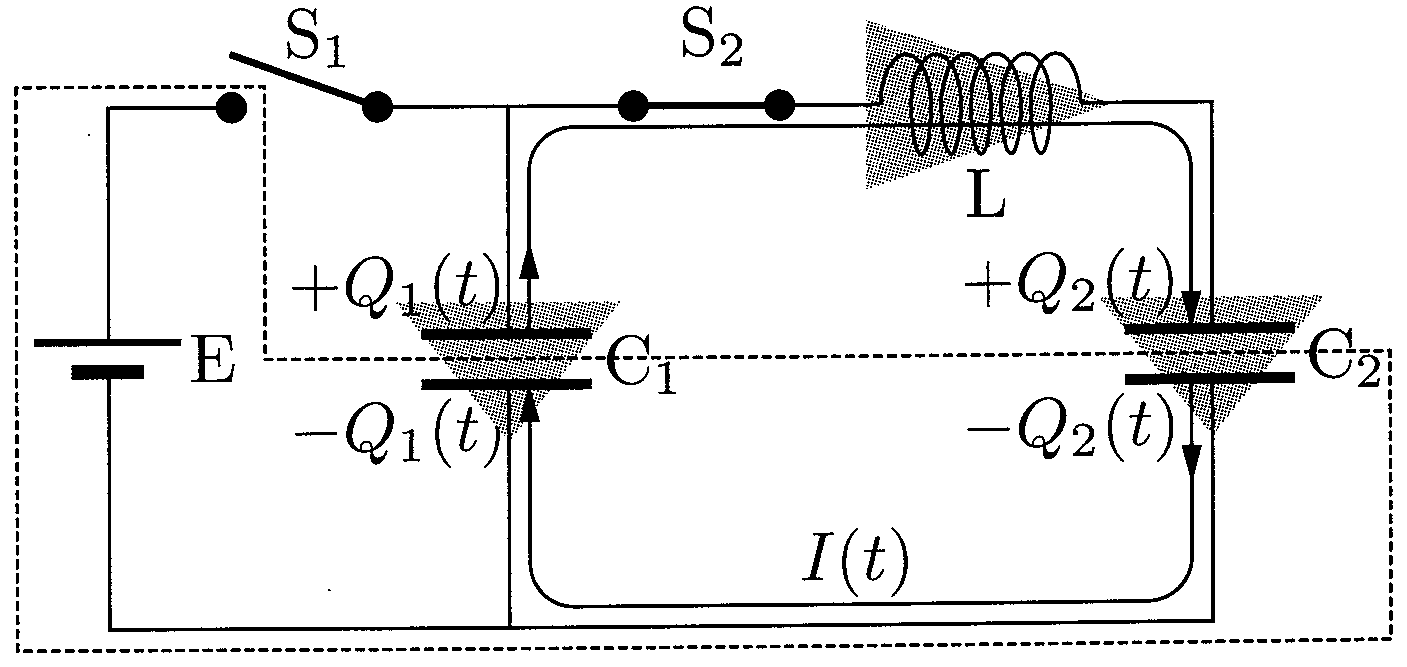
\includegraphics[keepaspectratio,width=58mm]{fig/n31_a118_zu.png}\end{center}
       点線枠内は外部とつながりを持たず，総電荷が保存される．$t=0$との間の電荷保存の法則より$-Q_0=-Q_1(t)-Q_2(t)$．整理して，
       \[Q_1(t)+Q_2(t)=CE\Ans\]
\ko{3} 極板へ流入する電流に着目して$\dfrac{d\{-Q_1(t)\}}{dt}=I(t)$，$\dfrac{d\{+Q_2(t)\}}{dt}=I(t)$．整理して，
       \[I(t)=-\frac{dQ_1(t)}{dt}=\frac{dQ_2(t)}{dt}\Ans\]
\ko{4} 右側ループにおいてキルヒホッフの第二法則より，
       \[-L\frac{dI}{dt}=-\frac{Q_1(t)}{C}+\frac{Q_2(t)}{C}\Ans\]
\ko{5} (3)を微分して$\dfrac{dI}{dt}=-\dfrac{d^2Q_1}{dt^2}$，(2)より$Q_2=CE-Q_1$．これらを(4)に代入して整理すると，
       \[\frac{d^2Q_1(t)}{dt^2}=-\frac{2}{LC}\Bigl\{Q_1(t)-\frac{CE}{2}\Bigr\}\]
       となる．これは，$Q_1(t)$が$\dfrac{CE}{2}$を中心として角周波数$\omega=\sqrt{\dfrac{2}{LC}}$で振動することを意味する．よって周期は
       \[T=\frac{2\pi}{\omega}=\pi\sqrt{2LC}\U{s}\Ans\]
\ko{6} 初期条件は$Q_1(0)=CE$，$I(0)=0$であり，$Q_1(t)$は$\dfrac{CE}{2}$を中心として振動するので，次図のようになる．
       \begin{center}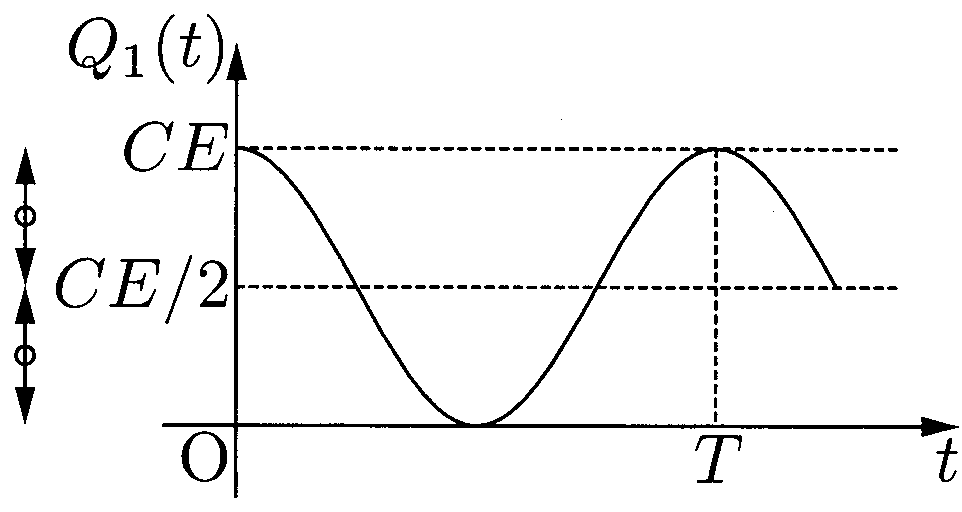
\includegraphics[keepaspectratio,width=46mm]{fig/n31_a118_graph.png}\end{center}
       振幅は$CE-\dfrac{CE}{2}=\dfrac{CE}{2}$で，最小値は$0$である．以上より，振動範囲は
       \[0\U{C}\sim CE\U{C}\Ans\]
\end{komon}

\MonN{119}{素子にかかる交流電圧と流れる交流電流の関係}\par\nopagebreak
\begin{sisin}
［117］は素子にかかる電圧から素子に流れる電流を計算する問題であったが，本問は逆に，素子に流れる電流から素子にかかる電圧を計算しようという問題である．考え方の基本は，素子にかかる電圧と電流の最大値・位相の間の関係式である．
% 原本は「B問題［31］」（旧回の番号）．
\end{sisin}
\KaiHead
各素子に対して流れている電流は$I(t)=I_0\sin\omega t$である．
\begin{komon}
\ko{1} 抵抗：$V_{\mathrm{R}0}=RI_0$で，電圧の位相は電流と同じ$\omega t$なので
       \[V_{\mathrm{R}}(t)=RI_0\sin\omega t\U{V}\Ans\]
\ko{2} コイル：$V_{\mathrm{L}0}=\omega LI_0$．電流の位相が電圧より$\dfrac{\pi}{2}$遅れる，すなわち電圧の位相は電流より$\dfrac{\pi}{2}$進むので
       \[\begin{aligned}V_{\mathrm{L}}(t)&=\omega LI_0\sin\Bigl(\omega t+\frac{\pi}{2}\Bigr)\\&=\omega LI_0\cos\omega t\U{V}\Ans\end{aligned}\]
\ko{3} コンデンサー：$V_{\mathrm{C}0}=\dfrac{I_0}{\omega C}$．電圧の位相は電流より$\dfrac{\pi}{2}$遅れるので
       \[\begin{aligned}V_{\mathrm{C}}(t)&=\frac{I_0}{\omega C}\sin\Bigl(\omega t-\frac{\pi}{2}\Bigr)\\&=-\frac{I_0}{\omega C}\cos\omega t\U{V}\Ans\end{aligned}\]
\end{komon}

\end{multicols}
